\documentclass[xcolor=table% ,aspectratio=169
,t]{beamer}
\usepackage[utf8]{inputenc}
\usepackage[T1]{fontenc}
\usepackage{xcolor}
\usepackage{colortbl}
\usepackage{graphicx}
\usepackage{booktabs,hhline}
\usepackage{grffile}
\usepackage[citestyle=authortitle,bibstyle=numeric,sorting=none]{biblatex}
\addbibresource{references.bib}

\makeatletter
\renewcommand\@makefnmark{\hbox{\@textsuperscript{\normalfont[\@thefnmark]}}}
\renewcommand\@makefntext[1]{{\normalfont[\@thefnmark]}\enspace #1}
\makeatother

\DeclareCiteCommand{\footfullcitetext}[\mkbibfootnotetext]
{\usebibmacro{prenote}}
{\usedriver
  {\DeclareNameAlias{sortname}{default}}
  {\thefield{entrytype}}}
{\multicitedelim}
{\usebibmacro{postnote}}

\usepackage{xpatch}
\xapptobibmacro{cite}{\setunit{\nametitledelim}\printfield{year}}{}{}
\usepackage{longtable}
\usepackage{array}
\usepackage{wrapfig}
\usepackage{rotating}
\usepackage[normalem]{ulem}
\usepackage{amsmath}
\usepackage{textcomp}
\usepackage{amssymb}
\usepackage{tikz}
\usetikzlibrary{patterns}
\usetikzlibrary{calc,math}
\usetikzlibrary{decorations.pathreplacing}
\usetikzlibrary{shapes,arrows}
\usetikzlibrary{shapes.geometric}
\usepackage{relsize}
\tikzset{fontscale/.style = {font=\relsize{#1}}}
\usepackage{marvosym}
\usepackage{multirow}
\usepackage{capt-of}
\usepackage{hyperref}
\usepackage{eurosym}
\usepackage[english]{babel}
\usepackage{textcomp}
\usepackage[space=true]{accsupp}
\usepackage{verbatim}
\usepackage{algorithm}
\usepackage{appendixnumberbeamer}
\usepackage[percent]{overpic}
\usepackage{geometry}
\usepackage{amsmath,mathtools,bussproofs,turnstile}
\usepackage{proof}
\usepackage{stmaryrd}
\usepackage[noend]{algpseudocode}
\usepackage[svgpath=results/]{svg}
\usepackage{import}
\usepackage{graphicx}
\usetheme[rounded,boxes,oldlogo,shadow]{ComputationalLogic}
\usepackage{pifont}% http://ctan.org/pkg/pifont
\usepackage{scalefnt}

\usepackage{presentation}

\newcommand{\cmark}{\ding{51}}%
\newcommand{\xmark}{\ding{55}}%

\newcommand{\SH}[1]{\begin{center} \textcolor{green!50!black}{#1} \end{center}}
\newcommand\MS[2][r]{\ifx t#1 \textcolor{blue}{[\textbf{MS:} #2]}
  \else \begin{center}\textcolor{blue}{\textbf{MS:} #2} \end{center} \fi}


\title[RL for Dynamic Strategies in \tct{}]{Reinforcement Learning for \newline Dynamic Strategies in \tct{}}

\author[Manuel Schneckenreither]{\textbf{Manuel Schneckenreither}
  \\[1.4ex] \footnotesize (supervised by Prof.\@ Dr.\@ Georg Moser)\\[2ex]
}

\location[]{CL Seminar}

% \authorrunning{Schneckenreither and Haeussler}
\institute{
  % Department of Information Systems,
  % Production and Logistics Management,
  University of Innsbruck, Austria
  % email: manuel.schneckenreither@uibk.ac.at
}

\date{Summer 2020}

% \setbeamertemplate{bibliography item}{\insertbiblabel}
% \setbeamertemplate{bibliography item}[text]

% \newcommand\hideit[1]{%
% \only<0| handout:1>{\mbox{}}%
% \invisible<0| handout:1>{#1}}

\begin{document}

\frame{\titlepage}

\begin{frame}[t]
  \frametitle{Motivation}

  \vspace{-1.5ex}
  \begin{block}{The Tyrolean Complexity Tool, i.e. \tct{}~\footnotemark}

    \begin{itemize}
    \item Automatic tool to infer runtime (and derivational) complexity
    \item Allows (first or higher-order) functional programs as generalised form of
      term rewrite systems as input
    \item In case of success: \tct{} outputs a certification proofing the presented asymptotic complexity
    \end{itemize}
  \end{block}\pause

  \begin{block}{Static Analyses}
    \begin{itemize}
    \item Static analyses are undecidable~\footnotemark{}
    \item Thus: Some sort of creativity is required (Strategies)
    \item Idea: Reinforcement learning for dynamic strategies
    \end{itemize}
  \end{block}


  \begin{centering}
    \footnotesize
    \addtocounter{footnote}{-2}
    \stepcounter{footnote}\footnotetext{\cite{schneckenreither2020dynamic}}
    \stepcounter{footnote}\footnotetext{\cite{landi1992undecidability}}

  \end{centering}


\end{frame}


\begin{frame}[t]
  \frametitle{\inserttitle{}}
  \begin{block}{Table of Contents}
    \vspace{0.2cm}
    \begin{enumerate}
    \item Motivation
    \item Discounted Reinforcement Learning (Discounted RL)
    \item Average Reward Adjusted Discounted RL
    \item Proposed Implementation in \tct{}
    \end{enumerate}
  \end{block}
\end{frame}

\section{Discounted Reinforcement Learning}
\label{sec:Discounted_Reinforcement_Learning}


\begin{frame}[t]
  \frametitle{Reinforcement Learning (RL)}

  \begin{block}{Reinforcement Learning Processes~\footnotemark}
    \centering
    % \only<1-1>{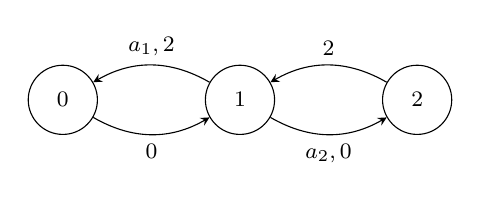
\begin{tikzpicture}[thin, scale=0.75]
  % Nodes
  \draw (-3,0) node(0) [circle,draw,minimum size=25] {\footnotesize \(0\)};
  \draw (0,0)  node(1) [circle,draw,minimum size=25] {\footnotesize \(1\)};
  \draw (3,0)  node(2) [circle,draw,minimum size=25] {\footnotesize \(2\)};

  % Edges
  \path[thin, ->, bend right, >=stealth] (1) edge[above] node {\footnotesize\(a_{1},2\)} (0);
  \path[thin, ->, bend right, >=stealth] (2) edge[above] node {\footnotesize\(2\)} (1);
  \path[thin, ->, bend right, >=stealth] (0) edge[below] node {\footnotesize\(\alert{0}\)} (1);
  \path[thin, ->, bend right, >=stealth] (1) edge[below] node {\footnotesize \(a_{2},\alert{0}\)} (2);

  % \draw (-1.5,0) node[] { A };
  % \draw (1.5,0) node[] { B };
\end{tikzpicture}

%%% Local Variables:
%%% mode: latex
%%% TeX-master: "../presentation"
%%% End:


}
    % \only<1->{
    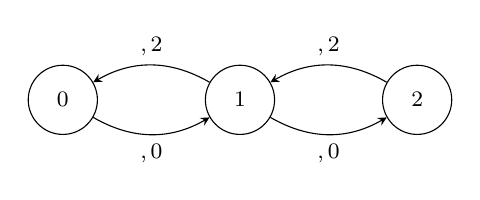
\begin{tikzpicture}[thin, scale=0.75]
  % Nodes
  \draw (-3,0) node(0) [circle,draw,minimum size=25] {\footnotesize \(0\)};
  \draw (0,0)  node(1) [circle,draw,minimum size=25] {\footnotesize \(1\)};
  \draw (3,0)  node(2) [circle,draw,minimum size=25] {\footnotesize \(2\)};

  % Edges
  \path[thin, ->, bend right, >=stealth] (1) edge[above] node {\footnotesize\(\lft,2\)} (0);
  \path[thin, ->, bend right, >=stealth] (2) edge[above] node {\footnotesize\(\lft,2\)} (1);
  \path[thin, ->, bend right, >=stealth] (0) edge[below] node {\footnotesize \(\rght,0\)} (1);
  \path[thin, ->, bend right, >=stealth] (1) edge[below] node {\footnotesize \(\rght,0\)} (2);

  % \draw (-1.5,0) node[] { A };
  % \draw (1.5,0) node[] { B };
\end{tikzpicture}

%%% Local Variables:
%%% mode: latex
%%% TeX-master: "../presentation"
%%% End:





    \begin{itemize}
      \only<1-1>{\item Based on dynamic programming: states, actions, rewards}
      % \only<2-3>{\item Markov Prop.: transitions with probability \(p(s_{t+1}, r_{t} \mid s_{t}, a_{t})\) }
      % \only<3-3>{\item RL processes: \textit{Markov decision processes} (MDPs)}
      \only<2-2>{
      \item Agent iteratively assesses state values
        % \(V_{\gamma}^{\pol_{\gamma}}(s) = \lim_{N \to \infty} E[\sum_{t=0}^{N-1} \gamma^{t} R_{t}^{\pol_{\gamma}}(s)]\)
        \(V_{\gamma}^{\pol}(s)\), where
      \item \(0 < \gamma < 1\) is the discount factor, \(\pol\) the policy function, and}
      \only<2-2>{\item for two consecutive observed states \(s_{t}, s_{t+1}\) with reward \(r_{t}\)
        \vspace{-5pt}
        \begin{align*}
          V^\pol_{\gamma}(s_{t}) \expSmth{\alpha} r_{t} + \gamma V^\pol_{\gamma}(s_{t+1})
        \end{align*}
      }
      \only<3-3>{
      \item Thus, state values \(V_{\gamma}^{\pol}(s)\) are
        \vspace{-5pt}
        \begin{align*}
          V_{\gamma}^{\pol}(s) = \lim_{N \to \infty} E[\sum_{t=0}^{N-1} \gamma^{t} R_{t}^{\pol}(s)]
        \end{align*}
        where \(R_{t}^{\pol}(s)\) the reward received at time \(t\) upon starting in state \(s\) by following policy \(\pol\). }
      \only<4->{
      \item RL in summary: Iteratively solving constraint problems composed of \(\size{\States}\)
        constraints and \(\size{\States}\) variables, where \(s \in \States\):
        \vspace{-5pt}
        \begin{align*}
          V^\pol_{\gamma}(0) & = 0 + \gamma V^\pol_{\gamma}(1) &  V^\pol_{\gamma}(2) & = 2 + \gamma V^\pol_{\gamma}(1) \\ 
          \lft\colon V^\pol_{\gamma}(1) & = 2 + \gamma V^\pol_{\gamma}(0) & \rght\colon V^\pol_{\gamma}(1) & = 0 + \gamma V^\pol_{\gamma}(2)
        \end{align*}
        % \only<8->{
        % \vspace{-1.1cm}
        % \begin{align*}
            %             \only<8-8>{\pol(1) = (p_{1}, p_{2})\colon}
            %     %             \only<8->{p_{1}a_{1} + p_{2}a_{2}\colon}
            %             & V^\pol_{\gamma}(1) = p_{1}(2 + \gamma V^\pol_{\gamma}(0)) + p_{2}(0 + \gamma V^\pol_{\gamma}(2))
                            %           \end{align*}
                            %                             }
      }
    \end{itemize}
  \end{block}
  \only<2-2>{
    \begin{minipage}{\textwidth}
      \centering
      \footnotesize (\(\expSmth{\alpha}\) is exp.\@ smoothed updating with rate \(\alpha\))
    \end{minipage}
  }
  \only<4->{
    \begin{minipage}{\textwidth}
      \centering
      \footnotesize (\(\size{\cdot}\) is the size of a set)
    \end{minipage}
  }

  % Citations
  \footnotetext{\cite{MillerVeinott1969}}

\end{frame}


\begin{frame}[t]
  \frametitle{Aim in Discounted Reinforcement Learning}

  \begin{block}{Aim of Discount Reinforcement Learning}
    \begin{itemize}
    \item Finding an optimal policy \(\polopt\)
    \item \(\polopt\) maximises the state value for all states \(s\) as compared to any other policy
      \(\pol\):
      \begin{align*}
        V_{\gamma}^{\polopt}(s) - V_{\gamma}^{\pol}(s) \geqslant 0
      \end{align*}
      \pause{}
    \item This criteria: discounted-optimality % (\(\gamma\)-optimality)
      as \(\gamma\) is \alert{fixed}
    \end{itemize}

  \end{block}


\end{frame}

\begin{frame}[t]

  % \frametitle{Example}
  \begin{block}{The issue of discounted-optimality illustrated~\footnotemark}

    \begin{figure}[t!]
      \centering
      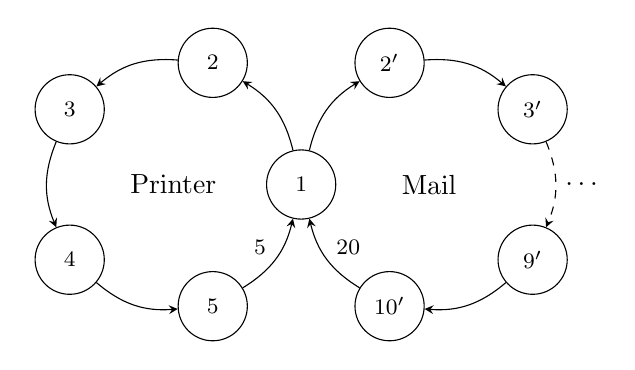
\begin{tikzpicture}[thin, scale=0.65]
  % Nodes
  \foreach \x in {1,...,5}{
    \draw ({cos(\x*72-72)*2.5},{sin(\x*72-72)*2.5}) node(\x) [circle,draw,minimum size=25] {\footnotesize \(\x\)};
  };
  \foreach[evaluate={
    \y=int(\x+5);
  }]  \x in {2,...,3}{
    \draw ({-cos(\x*72-72)*2.5+5},{sin(\x*72-72)*2.5}) node(\y) [circle,draw,minimum size=25]
    {\footnotesize \(\x'\)};
  };
  \foreach [evaluate={
    \y=int(\x+5);
    \z=int(\x+5);
  }] \x in {4,...,5}{
    \draw ({-cos(\x*72-72)*2.5+5},{sin(\x*72-72)*2.5}) node(\z) [circle,draw,minimum size=25]
    {\footnotesize \(\y'\)};
  };

  \newcommand\bend{22.5}
  % Edges
  \path[thin, ->, bend right=\bend, >=stealth] (1) edge[below left] node {\footnotesize\(\)} (2);
  \path[thin, ->, bend right=\bend, >=stealth] (2) edge[above]      node {\footnotesize\(\)} (3);
  \path[thin, ->, bend right=\bend, >=stealth] (3) edge[left ]      node {\footnotesize\(\)} (4);
  \path[thin, ->, bend right=\bend, >=stealth] (4) edge[above]      node {\footnotesize\(\)} (5);
  \path[thin, ->, bend right=\bend, >=stealth] (5) edge[above left] node[yshift=-2] {\footnotesize\(5\)} (1);

  \path[thin, ->, bend left=\bend, >=stealth]         (1)  edge[below right] node {\footnotesize\(\)} (7);
  \path[thin, ->, bend left=\bend, >=stealth]         (7)  edge[above right] node {\footnotesize\(\)} (8);
  \path[thin, ->, dashed, bend left=\bend, >=stealth] (8)  edge[right]       node {\(\ldots\)} (9) ;
  \path[thin, ->, bend left=\bend, >=stealth]         (9)  edge[above]       node {\footnotesize\(\)} (10);
  \path[thin, ->, bend left=\bend, >=stealth]         (10) edge[above right] node[yshift=-2] {\footnotesize\(20\)} (1);

  \draw (0,0) node[] { Printer };
  \draw (5,0) node[] { Mail };

\end{tikzpicture}

%%% Local Variables:
%%% mode: latex
%%% TeX-master: "../paper"
%%% End:


    \end{figure}
    \begin{itemize}

      % \only<1-1>{\item Assume that the agent has \(\infty\) time}
      \only<1->{\item Average reward received is
        \begin{itemize}
        \item \(1\) for the printer-loop
        \item \(2\) for the mail-loop
        \end{itemize}
        \only<2->{\item BUT\@: if \(\gamma < 3^{-\frac{1}{5}} \approx 0.8027\) the agent prefers the printer loop}}
    \end{itemize}


  \end{block}

  \footnotetext{Adapted from \cite{Mahadevan96_OptimalityCriteriaInReinforcementLearning}}

\end{frame}

\begin{frame}[t]
  \frametitle{Laurent Series Expansion of Discounted State Values}

  \begin{block}{Laurent Series Expansion of Discounted State Values\footnotemark}
    The Laurent series expansion of $V_{\gamma}^{\pol}(s)$ of discounted state values:
    \begin{align*}
      V_{\gamma}^{\pol}(s) =
      \frac{\only<1-1>{\alert{\avgrew^{\pol}}}\only<2->{\avgrew^{\pol}}}{1-\gamma} +
      \only<2-2>{\alert{V^{\pol}(s)}}\only<1-1>{V^{\pol}(s)}\only<3->{V^{\pol}(s)} +
      \only<1-2>{e_{\gamma}^{\pol}(s)}\only<3-3>{\alert{e_{\gamma}^{\pol}(s)}}\only<4->{e_{\gamma}^{\pol}(s)}
    \end{align*}
  \end{block}
  \only<1-2>{\footnotetext{\cite{MillerVeinott1969}}}
  \only<4->{\footnotetext{\cite{MillerVeinott1969}}}

  \only<1-1>{
    \begin{block}{Average Reward \(\avgrew^{\pol}\) (simplified for unichain Processes)}
      The \alert{average reward} is defined as
      \vspace{-2ex}
      \begin{align*}
        \avgrew^{\pol} = \lim_{N \to \infty} \frac{\E [\sum_{t=0}^{N-1}R_{t}^{\pol}]}{N}
      \end{align*}
      where \(R_{t}^{\pol}\) is the reward received at time \(t\).
    \end{block}
    % \begin{block}{Average Reward \(\avgrew^{\pol}\) (for unichain MDPs)}
    %   The \alert{average reward} is defined as
    %   \begin{align*}
    %     \avgrew^{\pol} = \avgrew^{\pol}(s) = \lim_{N \to \infty} \frac{\E [\sum_{t=0}^{N-1}R_{t}^{\pol}(s)]}{N}
    %   \end{align*}
    %   where \(R_{t}^{\pol}(s)\) is the reward received at time \(t\) starting in \(s\).
    % \end{block}
  }

  \only<2-2>{
    \begin{block}{Bias value \(V^{\pol}(s)\)}
      The \alert{bias value} is defined as
      \vspace{-2ex}
      \begin{align*}
        V^{\pol}(s) = \lim_{N \to \infty}{ \E [ \sum_{t=0}^{N-1}(R_{t}^{\pol}(s) - \avgrew^{\pol} )]}
      \end{align*}
      It is the additional reward that sums up when starting in state \(s\).
    \end{block}
  }

  \only<3-3>{
    \begin{block}{Error term of $e_{\gamma}^{\pol}$ \footnotemark{}}
      \alert{Error term} $e_{\gamma}^{\pol}(s)$ consists of infinitely many terms, but
      \vspace{-2ex}
      \begin{align*}
        \lim_{\gamma \to 1} e_{\gamma}^{\pol}(s) = 0
      \end{align*}
      If \(\gamma < 1\) it takes number of steps and reward values into account.
    \end{block}
    \footnotetext{\cite{Puterman94}}
  }
  % \only<5->{
  % \begin{block}{Note \only<5-5>{1}\only<6->{2}}
  %   \begin{enumerate}
  %     \only<5-5>{\item First term converges to infinity as \(\gamma\) increases.}
  %     \only<6->{
  %   \item First term: maximise average reward (gain-optimality)
  %   \item Second term: maximise bias value (bias-optimality)
  %   \item Third term: collect rewards as soon and in as little steps as possible
  %   }
  %   \end{enumerate}

  % \end{block}
  % }
  \only<5->{
    \begin{block}{Note}
      \begin{itemize}
      \item Recall: High \(\gamma \approx 1\) values required for optimal policies
      \item First term converges to \(\infty\) as \(\gamma \to 1\)
      \item Recall: RL is an iterative method
                            %                             \only<6->{
                            %                             \item First term: maximise average reward (gain-optimality)
                            %                             \item Second term: maximise bias value (bias-optimality)
                            %                             \item Third term: collect rewards as soon and in as little steps as possible
                            %                             }
      \end{itemize}

    \end{block}
  }
\end{frame}

\begin{frame}[t]
  \frametitle{So What?}

  \begin{block}{}
    \vspace{-2ex}
    \begin{alignat*}{1}
      V_{\gamma}^{\pol}(s) = \frac{\avgrew^{\pol}}{1-\gamma} + V^{\pol}(s) + e_{\gamma}^{\pol}(s)
    \end{alignat*}
  \end{block}

  \only<2-2>{
    \begin{block}{Consider this simple gridworld problem~\footnotemark}
      \begin{figure}[ht]
        \centering 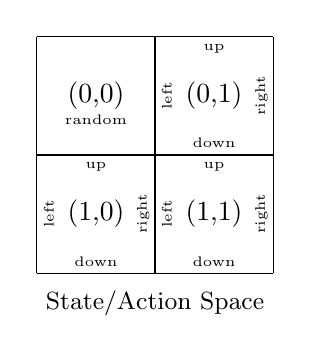
\begin{tikzpicture}[thin, scale=1.5]
  % Points
  \newcommand\maxX{1}         % = maxX
  \newcommand\maxY{1}         % = maxY
  \newcommand\goalX{0}         % = maxX
  \newcommand\goalY{0}         % = maxY

  \tikzmath{\maxXP = \maxX + 1; \maxYP = \maxY + 1;};

  \foreach \x in {0,...,\maxXP} {
    \foreach \y in {0,...,\maxYP} {
      \draw (\x,0) -- (\x,\maxYP) node[] {};
      \draw (0,\y) -- (\maxXP,\y) node[] {};
    }
  }
  \foreach \x in {0,...,\maxX} {
    \foreach \y in {0,...,\maxY} {
      \tikzmath{\xP = int(\maxX - \x); \yP = int(\maxY - \y);};
      \draw (\x+0.5, \y+0.5) node[] {(\yP,\x)};
      \draw (\x+0.5, \y+0.9) node[] (\yP,\x,up)                  {\ifthenelse{\x=\goalX \AND \yP=\goalY}{}{\tiny up   }};
      \draw (\x+0.5, \y+0.1) node[] (\yP,\x,down)                {\ifthenelse{\x=\goalX \AND \yP=\goalY}{}{\tiny down }};
      \draw (\x+0.1, \y+0.5) node[rotate=90] (\yP,\x,left)       {\ifthenelse{\x=\goalX \AND \yP=\goalY}{}{\tiny left }};
      \draw (\x+0.9, \y+0.5) node[rotate=90] (\yP,\x,right)      {\ifthenelse{\x=\goalX \AND \yP=\goalY}{}{\tiny right}};
    }
  }
  \draw (\goalX+0.5, \maxY-\goalY+0.3) node[] (\goalX,\goalY,rand) {\tiny random};

  % Name
  \draw (\maxXP/2, 0) node[below,minimum height=0.75cm] { \small State/Action Space};

\end{tikzpicture}
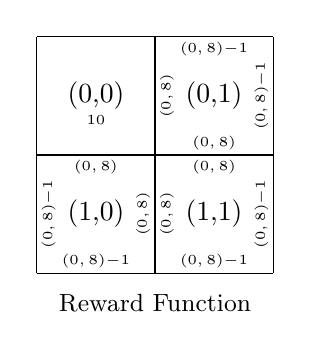
\begin{tikzpicture}[thin, scale=1.5]
  % Points
  \newcommand\maxX{1}         % = maxX
  \newcommand\maxY{1}         % = maxY
  \newcommand\goalX{0}         % = maxX
  \newcommand\goalY{0}         % = maxY

  \tikzmath{\maxXP = \maxX + 1; \maxYP = \maxY + 1;};

  \foreach \x in {0,...,\maxXP} {
    \foreach \y in {0,...,\maxYP} {
      \draw (\x,0) -- (\x,\maxYP) node[] {};
      \draw (0,\y) -- (\maxXP,\y) node[] {};
    }
  }
  \foreach \x in {0,...,\maxX} {
    \foreach \y in {0,...,\maxY} {
      \tikzmath{\xP = int(\maxX - \x); \yP = int(\maxY - \y);};
      \draw (\x+0.5, \y+0.5) node[] {(\yP,\x)};
      \draw (\x+0.5, \y+0.9) node[] (\yP,\x,up)                  {\ifthenelse{\x=\goalX \AND \yP=\goalY}{}{\tiny \(\Unif(0,8)\)\ifthenelse{\yP=0    }{\(-1\)}{} }};
      \draw (\x+0.5, \y+0.1) node[] (\yP,\x,down)                {\ifthenelse{\x=\goalX \AND \yP=\goalY}{}{\tiny \(\Unif(0,8)\)\ifthenelse{\yP=\maxY}{\(-1\)}{} }};
      \draw (\x+0.1, \y+0.5) node[rotate=90] (\yP,\x,left)       {\ifthenelse{\x=\goalX \AND \yP=\goalY}{}{\tiny \(\Unif(0,8)\)\ifthenelse{\x=0     }{\(-1\)}{} }};
      \draw (\x+0.9, \y+0.5) node[rotate=90] (\yP,\x,right)      {\ifthenelse{\x=\goalX \AND \yP=\goalY}{}{\tiny \(\Unif(0,8)\)\ifthenelse{\x=\maxX }{\(-1\)}{} }};
    }
  }
  \draw (\goalX+0.5, \maxY-\goalY+0.3) node[] (\goalX,\goalY,rand) {\tiny 10};

  % Name
  \draw (\maxXP/2, 0) node[below,minimum height=0.75cm] { \small Reward Function};

\end{tikzpicture}

%%% Local Variables:
%%% mode: latex
%%% TeX-master: "../paper"
%%% End:

      \end{figure}
    \end{block}
    \footnotetext{\tiny \cite{schneckenreither2020average}}
  }

  \only<3->{
    \begin{block}{Same problem as 5x5 grid}
      \begin{figure}[ht]
        \centering 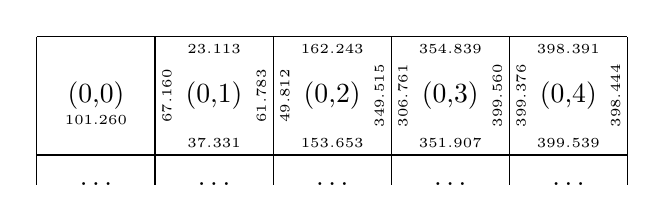
\begin{tikzpicture}[thin, scale=1.5]
  % Points
  \newcommand\maxX{4}         % = maxX
  \newcommand\maxY{0}         % = maxY
  \newcommand\goalX{0}         % = maxX
  \newcommand\goalY{0}         % = maxY

  \tikzmath{\maxXP = \maxX + 1; \maxYP = \maxY + 1;};

  \foreach \x in {0,...,\maxXP} {
    \foreach \y in {0,...,\maxYP} {
      \draw (\x,0) -- (\x,\maxYP) node[] {};
      \draw (0,\y) -- (\maxXP,\y) node[] {};
    }
    \draw (\x,0) -- (\x,-0.25) node[] {};
  }
  \foreach \x in {0,...,\maxX} {
    \draw (\x+0.5,-0.25) node[] (\x+0.5,-0.25) {\(\ldots\)};
  }

  % Node names
  \foreach \x in {0,...,\maxX} {
    \foreach \y in {0,...,\maxY} {
      \tikzmath{\xP = int(\maxX - \x); \yP = int(\maxY - \y);};
      \draw (\x+0.5, \y+0.5) node[] {(\yP,\x)};
    }
  }

  % goal state
  \draw (\goalX+0.5, \maxY-\goalY+0.3) node[] (\goalX,\goalY,rand) {\tiny 101.260};

  % x = 1; y=0
  \tikzmath{\x = 1; \y = 0; \xP = int(\maxX - \x); \yP = int(\maxY - \y);};
  \draw (\x+0.5, \y+0.9) node[] (\yP,\x,up)                  {\tiny \( 23.113 \)};
  \draw (\x+0.5, \y+0.1) node[] (\yP,\x,down)                {\tiny \( 37.331 \)};
  \draw (\x+0.1, \y+0.5) node[rotate=90] (\yP,\x,left)       {\tiny \( 67.160 \)};
  \draw (\x+0.9, \y+0.5) node[rotate=90] (\yP,\x,right)      {\tiny \( 61.783 \)};

  % x = 2; y=0
  \tikzmath{\x = 2; \y = 0; \xP = int(\maxX - \x); \yP = int(\maxY - \y);};
  \draw (\x+0.5, \y+0.9) node[] (\yP,\x,up)                  {\tiny \( 162.243 \)};
  \draw (\x+0.5, \y+0.1) node[] (\yP,\x,down)                {\tiny \( 153.653 \)};
  \draw (\x+0.1, \y+0.5) node[rotate=90] (\yP,\x,left)       {\tiny \( 49.812  \)};
  \draw (\x+0.9, \y+0.5) node[rotate=90] (\yP,\x,right)      {\tiny \( 349.515 \)};

  % x = 3; y=0
  \tikzmath{\x = 3; \y = 0; \xP = int(\maxX - \x); \yP = int(\maxY - \y);};
  \draw (\x+0.5, \y+0.9) node[] (\yP,\x,up)                  {\tiny \( 354.839 \)};
  \draw (\x+0.5, \y+0.1) node[] (\yP,\x,down)                {\tiny \( 351.907 \)};
  \draw (\x+0.1, \y+0.5) node[rotate=90] (\yP,\x,left)       {\tiny \( 306.761 \)};
  \draw (\x+0.9, \y+0.5) node[rotate=90] (\yP,\x,right)      {\tiny \( 399.560 \)};

  % x = 4; y=0
  \tikzmath{\x = 4; \y = 0; \xP = int(\maxX - \x); \yP = int(\maxY - \y);};
  \draw (\x+0.5, \y+0.9) node[] (\yP,\x,up)                  {\tiny \( 398.391 \)};
  \draw (\x+0.5, \y+0.1) node[] (\yP,\x,down)                {\tiny \( 399.539 \)};
  \draw (\x+0.1, \y+0.5) node[rotate=90] (\yP,\x,left)       {\tiny \( 399.376 \)};
  \draw (\x+0.9, \y+0.5) node[rotate=90] (\yP,\x,right)      {\tiny \( 398.444 \)};

  % Name
  % \draw (\maxXP/2, -0.25) node[below,minimum height=0.75cm] { \small Estimated \(Q_{\gamma_{1}}^{\pol}(s,a)\) values};
\end{tikzpicture}

%%% Local Variables:
%%% mode: latex
%%% TeX-master: "../paper"
%%% End:

      \end{figure}
      \vspace{-2.1ex}
      \begin{itemize}
      \item All states values completely assessed independently
      \item For \(\gamma \approx 1\colon \avgrew^{\pol} / (1-\gamma) \gg V^{\pol}(s) + e_{\gamma}^{\pol}(s)\)
      \item Thus, all values need to increase to \( \approx \avgrew^{\pol} / (1-\gamma)\)
      \item BUT\@: Greater \(V_{\gamma}^{\pol}(s)\), then more likely to be picked
      \end{itemize}

    \end{block}
  }

\end{frame}


\section{Average Reward Adjusted Discounted Reinforcement Learning}
\label{sec:Average_Reward_Adjusted_Discounted_Reinforcement_Learning}


\begin{frame}[t]
  \frametitle{Average Reward Adjusted Reinforcement Learning}

  \begin{block}{Basic Idea}
    Separately assessing
    \begin{itemize}
    \item average reward \(\avgrew^{\pol}\)
    \item bias value \(V^{\pol}(s)\)
    \end{itemize}
  \end{block}\pause

  \begin{block}{Algorithm}
    \vspace{-2ex}
    \begin{align*}
      \avgrew^{\pol}  & \expSmth{\alpha} r_{t} + V^\pol(s_{t+1}) - V^\pol(s_{t})\\
      V^\pol(s_{t}) & \expSmth{\beta} r_{t} + \gamma_{1} V^\pol(s_{t+1}) - \avgrew^{\pol}
    \end{align*}
    Note: We can set \(\gamma_{1} = 1\) here, as the subtraction of the average reward bounds the
    state values.
  \end{block}
\end{frame}


\begin{frame}
  \frametitle{Discounted vs. Average Reward Adjusted RL}
  \begin{block}{Reconsider the 5x5 Gridworld~\footnotemark}
    \centering
                      %                       \ratab{}
    \begin{tabular}{@{}lrcr@{}}
      \toprule
      % \multirow{2}{*}{\textbf{Gridworld}} & \multicolumn{2}{c}{Sum Reward}  &
      % \multicolumn{2}{c}{Avg.\@ Steps to Goal}\\
      Algorithm & \multicolumn{1}{c}{Sum Reward}  & &\multicolumn{1}{c}{Avg.\@ Steps}\\
      % \cmidrule(r){2-3} \cmidrule(l){4-5}
      % Algorithm & Mean & Mean\\
      \midrule
      \ARA{} \(\gamma_1=0.99\)  & \cellcolor{gr}\(\textbf{51894.094}\) & & \(\textbf{5.039}\)\\
      \ARA{} \(\gamma_1=0.999\) & \cellcolor{gr}\(51878.069\)          & & \cellcolor{gr}\(5.063\)\\
      \ARA{} \(\gamma_1=1.00\)  & \cellcolor{gr}\(51856.529\)          & & \cellcolor{gr}\(5.055\)\\
      \hhline{|~|-|~|-|}
      \QL{}  \(\gamma=0.99\)  & \cellcolor{gr2}\(34409.464\)         & & \cellcolor{gr2}\(7661.833\)  \\
      \QL{}  \(\gamma=0.999\) & \cellcolor{gr2}\(33931.917\)         & & \cellcolor{gr2}\(7379.155\) \\
      \QL{}  \(\gamma=0.50\)  & \(30171.837\)                        & &  \(9999.000\)\\
      \bottomrule
    \end{tabular}\\[0.5em]
            %             \begin{itemize}
    \begin{minipage}{\textwidth}
      \centering
      {\footnotesize (\(500k\) learning steps, \(40 \times 10k\) greedy evaluation steps)}

    \end{minipage}

            %             \caption{\label{tbl:grid} The results of the gridworld example, where all \ARA{} instances
            %             inferred an average reward of \(\avgrew^{\pol}=5.215\)}
  \end{block}
  \footnotetext{\cite{schneckenreither2020average}}
\end{frame}


\begin{frame}[t]
  \frametitle{Average Reward Adjusted Reinforcement Learning}

  \begin{block}{More Insights} Average Reward Adjusted Reinforcement Learning \(\ldots\)
    \begin{enumerate}
    \item requires fewer number of learning steps
    \item allows more natural specification of reward function (continuous feedback), which helps
      to
      \begin{itemize}
      \item find the goal
      \item distinguish between good and bad sequences of actions \only<2-2>{
          \begin{minipage}{0.7\textwidth} \centering
            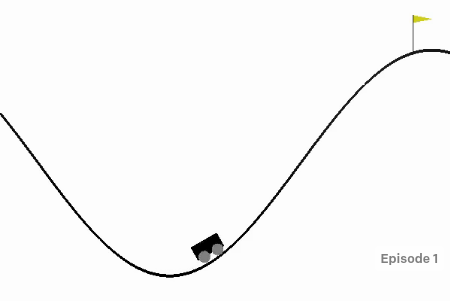
\includegraphics[width=0.5\textwidth]{figures/mountaincar.png}\\ {\tiny Source:
              https://gym.openai.com/}
          \end{minipage} }
      \end{itemize}
    \end{enumerate}
  \end{block}
\end{frame}

\begin{frame}[t]
  \frametitle{Average Reward Adjusted Reinforcement Learning}

  \begin{block}{More Insights (cont'd)}
    Average Reward Adjusted Reinforcement Learning \(\ldots\)
    \begin{enumerate}
    \item[3.] state values are easier to interpret
    \item[4.] normed state values have a higher spread
      \begin{itemize}
      \item important when approximating the state-value function (ANN)
      \end{itemize}
    \end{enumerate}
  \end{block}
\end{frame}


% \section{Proposed Implementation in \tct{}}


\begin{frame}
  \frametitle{Implementation in \tct{}}

  \begin{block}{Process Schema~\footnotemark}
    \centering
    \resizebox{0.9\linewidth}{!}{\begin{tikzpicture}
  [state/.style={circle,draw,minimum size=12ex,inner sep=0.075cm}
  , scale=1.0
  , thin]

  \draw (00ex, 00ex) node[state,minimum size=6ex] (s0) {\(\cdot\)};
  \draw (25ex, 00ex) node[state] (s1) {\(s\)};
  \draw (50ex, 00ex) node[state] (s2) {\( s \seq{} \)};
  \draw (75ex, 00ex) node[state,ellipse,dashed] (s3) {\( s \seq{} t\)};
  \draw (25ex,-15ex) node[state,ellipse,dashed] (s4) {\( s \alter{} \mathsf{identity}\)};
  \draw (75ex,-15ex) node[state,minimum size=6ex,fill] (se) {\(\cdot\)};

  % Paths
  \path (s0) edge[->] node[align=left,above] {\(\small \mathsf{strat\colon identity}\)} (s1); 
  \path (s1) edge[->] node[align=left,above] {\(\small \Seq\)} (s2);
  \path (s2) edge[->] node[align=left] {\(\small{\mathsf{Concrete}}\)\\ \(\small{\mathsf{Method}}\)} (s3); 
  \path (s3) edge[->,bend right] node[align=left, above] {\small Progress reward} (s1); 
  \path (s1) edge[->,bend left] node[align=left,right] {\(\small \Alt\)} (s4.east); 
  \path (s4.west) edge[->,bend left] node[align=left,left] {} (s1); 
  \path (s1) edge[->,near end] node[align=left,sloped] {\(\small \End\) \\ \small Final reward} (se); 
  
\end{tikzpicture}


%%% Local Variables:
%%% mode: latex
%%% TeX-master: "../presentation"
%%% End:
}
    \begin{itemize}
    \item Starting strategy: identity
    \item Strategy operators: Sequencing \(\seq\) and alternative \(\alter\)
    \item Two agents: decomposition and complexity analyser
    \end{itemize}
  \end{block}
  \footnotetext{\cite{schneckenreither2020dynamic}}
\end{frame}

\begin{frame}
  \frametitle{Implementation in \tct{}}

  \begin{block}{Binary Strategy Tree~\footnotemark}
    \centering
    \resizebox{0.8\linewidth}{!}{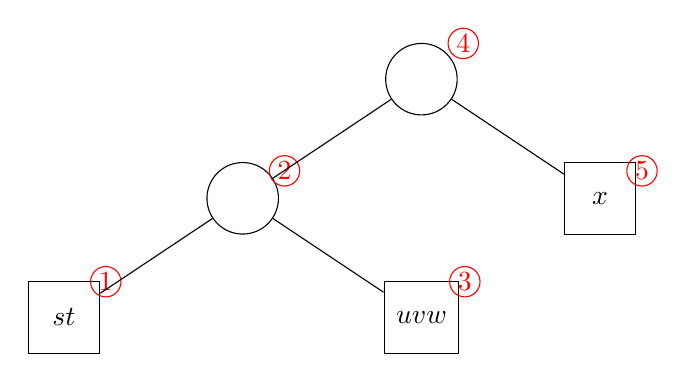
\begin{tikzpicture}
  [state/.style={circle,draw,minimum size=12ex,inner sep=0.075cm}
  ,leaf/.style={rectangle,draw,minimum size=12ex,inner sep=1ex}
  ,nr/.style={circle,red,draw,yshift=3ex,xshift=2pt,inner sep=1pt}
  , scale=1
  , thin]

  \draw (00ex,  00ex) node[state,minimum size=6ex]  (s0) {\(\alter\)};
  \draw (-15ex, -10ex) node[state,minimum size=6ex] (s1) {\(\alter\)};
  \draw (-30ex, -20ex) node[leaf,minimum size=6ex]  (s2) {\(s \seq t\)};
  \draw ( 00ex, -20ex) node[leaf,minimum size=6ex]  (s3) {\(u \seq v \seq w\)};
  \draw ( 15ex, -10ex) node[leaf,minimum size=6ex]  (s4) {\(x\)};

  \draw (s2.east) node[nr]  () {\(\scalefont{0.05} 1\)};
  \draw (s1.east) node[nr,yshift=-3pt]  () {\(\scalefont{0.05} 2\)};
  \draw (s3.east) node[nr]  () {\(\scalefont{0.05} 3\)};
  \draw (s0.east) node[nr]  () {\(\scalefont{0.05} 4\)};
  \draw (s4.east) node[nr,yshift=-3pt]  () {\(\scalefont{0.05} 5\)};

  % Paths
  \path (s0) edge[] node[align=left,above] {} (s1);
  \path (s1) edge[] node[align=left,above] {} (s2);
  \path (s1) edge[] node[align=left,above] {} (s3);
  \path (s0) edge[] node[align=left,above] {} (s4);

\end{tikzpicture}


%%% Local Variables:
%%% mode: latex
%%% TeX-master: "../presentation"
%%% End:
}
    \begin{itemize}
    \item No ambiguity by enforcing right-associativity of \(\alter\)
      % Starting strategy: identity
      % \item Strategy operators: Sequencing \(\seq\) and alternative \(\alter\)
      % \item Two agents: decomposition and complexity analyser
    \end{itemize}
  \end{block}
  \footnotetext{\cite{schneckenreither2020dynamic}}
\end{frame}


\begin{frame}
  \frametitle{Implementation in \tct{}}

  \begin{block}{State Space}
    \begin{itemize}
    \item Characteristics of input problem, e.g.
      \begin{itemize}
      \item number of rules
      \item number of (root) symbols
      \item left-linearity, right-linearity
      \end{itemize}
    \item Representation of current strategy 
      \begin{itemize}
      \item Counter specifying steps until last occurrence of concrete method
      \end{itemize}
    \end{itemize}
  \end{block}
  \footnotetext{\cite{schneckenreither2020dynamic}}
\end{frame}

\begin{frame}
  \frametitle{Conclusion}

  \begin{block}{Summary}
    \begin{itemize}
    \item Discounted Reinforcement Learning
    \item Average Reward Adjusted Discounted Reinforcement Learning
    \item Implementation Idea for Dynamic Strategies in \tct{}
    \end{itemize}
  \end{block}\pause

  % \begin{block}{Reality...}
  %   \begin{itemize}
  %   \item Algorithm is more complex, e.g.\@ incorporates the error term
  %   \item Artificial Neural Network (ANN) to approximate value function
  %   \item \(\ldots\)
  %   \end{itemize}
  % \end{block}
  
  \begin{block}{}
    \centering
    Thank you for your attention!
  \end{block}


\end{frame}

\appendix

\begin{frame}

\end{frame}

\begin{frame}
  \frametitle{Implementation in \tct{}}

  \begin{block}{Reward Function~\footnotemark}
    Assume current strategy \(s_{t}\) at step \(t\), a timeout of \(T\) seconds, a measured
    execution time of \(t' \leqslant T\) seconds and resulting polynomial complexity \(C\):
    \begin{align*}
      r(s_{t}) =
      \begin{cases}
        c T + t'    & \qquad   \text{if $C$ is }\bO(n^{c}) \text{ and } c < P_{\max{}}\\
        P_{\max{}} T & \qquad \text{otherwise}
      \end{cases}
    \end{align*}
    where \(P_{\max{}}\) is the maximum polynomial degree being considered.
  \end{block}

  \footnotetext{\cite{schneckenreither2020dynamic}}
\end{frame}


\begin{frame}[t]
  \frametitle{Reinforcement Learning (RL)}

  \begin{block}{Markov Decision Processes~\footnotemark}
    \centering
    % \only<1-1>{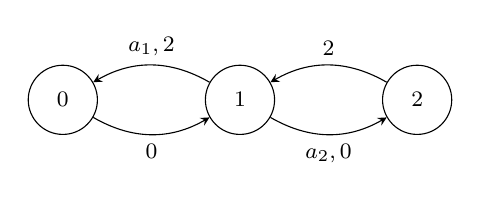
\begin{tikzpicture}[thin, scale=0.75]
  % Nodes
  \draw (-3,0) node(0) [circle,draw,minimum size=25] {\footnotesize \(0\)};
  \draw (0,0)  node(1) [circle,draw,minimum size=25] {\footnotesize \(1\)};
  \draw (3,0)  node(2) [circle,draw,minimum size=25] {\footnotesize \(2\)};

  % Edges
  \path[thin, ->, bend right, >=stealth] (1) edge[above] node {\footnotesize\(a_{1},2\)} (0);
  \path[thin, ->, bend right, >=stealth] (2) edge[above] node {\footnotesize\(2\)} (1);
  \path[thin, ->, bend right, >=stealth] (0) edge[below] node {\footnotesize\(\alert{0}\)} (1);
  \path[thin, ->, bend right, >=stealth] (1) edge[below] node {\footnotesize \(a_{2},\alert{0}\)} (2);

  % \draw (-1.5,0) node[] { A };
  % \draw (1.5,0) node[] { B };
\end{tikzpicture}

%%% Local Variables:
%%% mode: latex
%%% TeX-master: "../presentation"
%%% End:


}
    % \only<1->{
    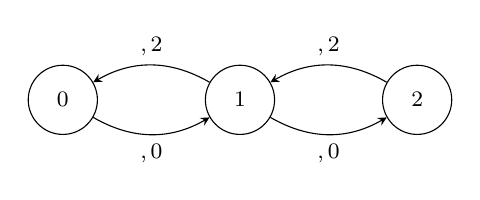
\begin{tikzpicture}[thin, scale=0.75]
  % Nodes
  \draw (-3,0) node(0) [circle,draw,minimum size=25] {\footnotesize \(0\)};
  \draw (0,0)  node(1) [circle,draw,minimum size=25] {\footnotesize \(1\)};
  \draw (3,0)  node(2) [circle,draw,minimum size=25] {\footnotesize \(2\)};

  % Edges
  \path[thin, ->, bend right, >=stealth] (1) edge[above] node {\footnotesize\(\lft,2\)} (0);
  \path[thin, ->, bend right, >=stealth] (2) edge[above] node {\footnotesize\(\lft,2\)} (1);
  \path[thin, ->, bend right, >=stealth] (0) edge[below] node {\footnotesize \(\rght,0\)} (1);
  \path[thin, ->, bend right, >=stealth] (1) edge[below] node {\footnotesize \(\rght,0\)} (2);

  % \draw (-1.5,0) node[] { A };
  % \draw (1.5,0) node[] { B };
\end{tikzpicture}

%%% Local Variables:
%%% mode: latex
%%% TeX-master: "../presentation"
%%% End:





    \begin{itemize}
      \item Based on dynamic programming: states, actions, rewards
      \item Markov Prop.: transitions with probability \(p(s_{t+1}, r_{t} \mid s_{t}, a_{t})\) 
      \item RL processes: \textit{Markov decision processes} (MDPs)
    \end{itemize}
  %     \only<4-5>{
  %     \item Agent iteratively assesses state values
  %       % \(V_{\gamma}^{\pol_{\gamma}}(s) = \lim_{N \to \infty} E[\sum_{t=0}^{N-1} \gamma^{t} R_{t}^{\pol_{\gamma}}(s)]\)
  %       \(V_{\gamma}^{\pol}(s)\), where
  %     \item \(0 < \gamma < 1\) is the discount factor, \(\pol\) the policy function, and}
  %     \only<5-5>{\item for two consecutive observed states \(s_{t}, s_{t+1}\) with reward \(r_{t}\)
  %       \vspace{-5pt}
  %       \begin{align*}
  %         V^\pol_{\gamma}(s_{t}) \expSmth{\alpha} r_{t} + \gamma V^\pol_{\gamma}(s_{t+1})
  %       \end{align*}
  %     }
  %     \only<6-6>{
  %     \item Thus, state values \(V_{\gamma}^{\pol}(s)\) are
  %       \vspace{-5pt}
  %       \begin{align*}
  %         V_{\gamma}^{\pol}(s) = \lim_{N \to \infty} E[\sum_{t=0}^{N-1} \gamma^{t} R_{t}^{\pol}(s)]
  %       \end{align*}
  %       where \(R_{t}^{\pol}(s)\) the reward received at time \(t\) upon starting in state \(s\) by following policy \(\pol\). }
  %     \only<7->{
  %     \item RL in summary: Iteratively solving constraint problems composed of \(\size{\States}\)
  %       constraints and \(\size{\States}\) variables, where \(s \in \States\):
  %       \vspace{-5pt}
  %       \begin{align*}
  %         V^\pol_{\gamma}(0) & = 0 + \gamma V^\pol_{\gamma}(1) &  V^\pol_{\gamma}(2) & = 2 + \gamma V^\pol_{\gamma}(1)
  %                                                                                      \only<7-7>{\\ a_{1}\colon V^\pol_{\gamma}(1) & = 2 + \gamma V^\pol_{\gamma}(0) & a_{2}\colon V^\pol_{\gamma}(1) & = 0 + \gamma V^\pol_{\gamma}(2)}
  %       \end{align*}
  %       % \only<8->{
  %       % \vspace{-1.1cm}
  %       % \begin{align*}
  %           %             \only<8-8>{\pol(1) = (p_{1}, p_{2})\colon}
  %           %     %             \only<8->{p_{1}a_{1} + p_{2}a_{2}\colon}
  %           %             & V^\pol_{\gamma}(1) = p_{1}(2 + \gamma V^\pol_{\gamma}(0)) + p_{2}(0 + \gamma V^\pol_{\gamma}(2))
  %                           %           \end{align*}
  %                           %                             }
  %     }
  %   \end{itemize}
  \end{block}
  % \only<5-5>{
  %   \begin{minipage}{\textwidth}
  %     \centering
  %     \footnotesize (\(\expSmth{\alpha}\) is exp.\@ smoothed updating with rate \(\alpha\))
  %   \end{minipage}
  % }
  % \only<7->{
  %   \begin{minipage}{\textwidth}
  %     \centering
  %     \footnotesize (\(\size{\cdot}\) is the size of a set)
  %   \end{minipage}
  % }

  % Citations
  \footnotetext{\cite{MillerVeinott1969}}

\end{frame}


\begin{frame}[t]
  \frametitle{Motivation: More Applications}

  % \begin{block}{Problems in Operation Research Domain}
  %   \begin{itemize}
  %   \item Periodic and discrete decisions
  %   \item Maximizing profits
  %   \item High degree of complexity
  %   \end{itemize}
  % \end{block}

  \vspace{-1.5ex}
  \begin{block}{}

    \hspace*{-1.4ex}\begin{tikzpicture}[queue/.style={regular polygon,regular polygon sides=4,inner sep=0.075cm},scale=0.8]

  \draw (-3.5,0) node[] {$\ldots$};
  \draw (-4.1,-1.75) node[] {\scriptsize Due Date:};

  \draw (-3.0,-1.5) -- (-3.0,1.5)
        (-2.5,1.5)  -- (-2.5,-1.5)
        (-2.5,-1.5) -- (-3.0,-1.5);
  \draw (-2.75,-1.75) node[] {\tiny $t+3$};

  \draw (-2.5,-1.5) -- (-2.5,1.5)
        (-2,1.5)  -- (-2,-1.5)
        (-2,-1.5) -- (-2.5,-1.5);
  \draw (-2.25,-2) node[] {\tiny $t+2$};
  \draw (-2 ,-1.5) -- (-2,1.5)
        (-1.5,1.5)  -- (-1.5,-1.5)
        (-1.5,-1.5) -- (-2,-1.5);
  \draw (-1.75,-1.75) node[] {\tiny $t+1$};

  \draw (-1.5,0.0) node[] (OP) {};
  % \draw [decorate,decoration={brace,amplitude=5pt},xshift=-2pt,yshift=0pt] (-1.0,-2.25) -- (-3.75,-2.25)     node [black,midway,yshift=-0.4cm] {\scriOrder Pool};
  % \draw [decorate,decoration={brace,amplitude=5pt},xshift=-2pt,yshift=0pt] (5.0,-2.25) -- (-.75,-2.25)  node [black,midway,yshift=-0.4cm] {Production System};
  % \draw [decorate,decoration={brace,amplitude=5pt},xshift=-2pt,yshift=0pt] (7,-2.25) -- (5.25,-2.25) node [black,midway,yshift=-0.4cm] {Inventory};

  % \draw (-1.75,-1.3) node[circle,inner sep=1pt,minimum size=0.2cm,draw] {$\scriptscriptstyle 1$};
  % \draw (-1.75,-1.0) node[circle,inner sep=1pt,minimum size=0.2cm,draw] {$\scriptscriptstyle 1$};
  % \draw (-1.75,-0.7) node[circle,inner sep=1pt,minimum size=0.2cm,draw] {$\scriptscriptstyle 2$};
  % \draw (-1.75,-0.4) node[circle,inner sep=1pt,minimum size=0.2cm,draw] {$\scriptscriptstyle 2$};
  % \draw (-1.75,-0.1) node[circle,inner sep=1pt,minimum size=0.2cm,draw] {$\scriptscriptstyle 3$};
  % \draw (-1.75, 0.2) node[circle,inner sep=1pt,minimum size=0.2cm,draw] {$\scriptscriptstyle 3$};
  % \draw (-1.75, 0.5) node[circle,inner sep=1pt,minimum size=0.2cm,draw] {$\scriptscriptstyle 4$};
  % \draw (-1.75, 0.8) node[circle,inner sep=1pt,minimum size=0.2cm,draw] {$\scriptscriptstyle 4$};
  % \draw (-1.75, 1.1) node[circle,inner sep=1pt,minimum size=0.2cm,draw] {$\scriptscriptstyle 6$};
  % \draw (-1.75, 1.4) node[circle,inner sep=1pt,minimum size=0.2cm,draw] {$\scriptscriptstyle 6$};
  % \draw (-1.75, 1.7) node[circle,inner sep=1pt,minimum size=0.2cm,draw] {$\scriptscriptstyle 6$};

  \draw (-2.25,-1.3) node[circle,inner sep=1pt,minimum size=0.2cm,draw] {$  \scriptscriptstyle 1$};
  \draw (-2.25,-0.95) node[circle,inner sep=1pt,minimum size=0.2cm,draw] {$ \scriptscriptstyle 2$};
  \draw (-2.25,-0.6) node[circle,inner sep=1pt,minimum size=0.2cm,draw] {$  \scriptscriptstyle 1$};
  \draw (-2.25,-0.25) node[circle,inner sep=1pt,minimum size=0.2cm,draw] {$ \scriptscriptstyle 1$};

  \draw (-2.75,-1.3) node[circle,inner sep=1pt,minimum size=0.2cm,draw] {$  \scriptscriptstyle 1$};
  \draw (-2.75,-0.95) node[circle,inner sep=1pt,minimum size=0.2cm,draw] {$ \scriptscriptstyle 1$};
  \draw (-2.75,-0.6) node[circle,inner sep=1pt,minimum size=0.2cm,draw] {$  \scriptscriptstyle 2$};
  \draw (-2.75,-0.25) node[circle,inner sep=1pt,minimum size=0.2cm,draw] {$ \scriptscriptstyle 2$};
  \draw (-2.75, 0.1) node[circle,inner sep=1pt,minimum size=0.2cm,draw] {$  \scriptscriptstyle 2$};
  \draw (-2.75, 0.45) node[circle,inner sep=1pt,minimum size=0.2cm,draw] {$ \scriptscriptstyle 1$};
  \draw (-2.75, 0.8) node[circle,inner sep=1pt,minimum size=0.2cm,draw] {$  \scriptscriptstyle 2$};

  \draw (0.7,0)    node[minimum size=1cm,draw,align=center] (M1) {WC1\\[-1ex]{\tiny $\Unif(70,130)$}};
  \draw (3.45,0.75)   node[minimum size=1cm,draw,align=center] (M2) {WC2\\[-1ex]{\tiny  $\Unif(130,170)$}};
  \draw (3.45,-0.75)  node[minimum size=1cm,draw,align=center] (M3) {WC3\\[-1ex]{\tiny $\Unif(180,200)$}};
  % \draw (6,1.5)    node[minimum size=1cm,draw,align=center] (M4) {M4\\[-1ex]{\tiny $\Exp(210)$ or}\\[-1ex]{\tiny $\Unif(50,370)$}};
  % \draw (6,0)      node[minimum size=1cm,draw,align=center] (M5) {M5\\[-1ex]{\tiny $\Exp(285)$ or}\\[-1ex]{\tiny $\Unif(200,370)$}};
  % \draw (6,-1.5)   node[minimum size=1cm,draw,align=center] (M6) {M6\\[-1ex]{\tiny $\Exp(215)$ or}\\[-1ex]{\tiny $\Unif(110,320)$}};
  \draw (6,0)      node[minimum size=1cm,draw,align=center,fill] (\fgi{}) {\color{white} \fgi{}};

  \draw (M1.west) node[draw,queue,minimum size=0.05cm,fill,xshift=-0.075cm] (Q1) {};
  \draw (M2.west) node[draw,queue,minimum size=0.05cm,fill,xshift=-0.075cm] (Q2) {};
  \draw (M3.west) node[draw,queue,minimum size=0.05cm,fill,xshift=-0.075cm] (Q3) {};
  % \draw (M4.west) node[draw,queue,minimum size=0.05cm,fill,xshift=-0.075cm] (Q4) {};
  % \draw (M5.west) node[draw,queue,minimum size=0.05cm,fill,xshift=-0.075cm] (Q5) {};
  % \draw (M6.west) node[draw,queue,minimum size=0.01cm,fill,xshift=-0.075cm] (Q6) {};

  \draw (8.5, 1) node[] (CustomerTop) {\Huge \Gentsroom};
  \draw (8, 0.5) node[] {\Huge \Ladiesroom};
  \draw (8.5, 0) node[] (Customer) {\Huge \Gentsroom};
  \draw (8,-0.5) node[] {\Huge \Ladiesroom};
  \draw (8.5,-1) node[] {\Huge \Gentsroom};

  % Paths
  \path (OP.center) edge[->, bend left=10]
  node[xshift=0.088cm,yshift=0.12cm,align=center] {\scriptsize \alert{Order} \\[-1ex] \scriptsize
    \alert{Release} \\[1.05ex] \scriptsize % \alert{via LT}
  } (Q1);

  
  \path (M1) edge[->, bend left=10, above]                 node[xshift=-0.1cm,yshift=-0.05cm] {$\scriptstyle % \text{P}1
    $} (Q2);
  \path (M1) edge[->, bend right=10,above]                 node[xshift=0.1cm,yshift=-0.05cm] {$\scriptstyle % \text{P}2
    $} (Q3);
  % \path (M2) edge[->, bend left=10,above,near start ]      node {$\scriptstyle 1$}     (Q4);
  % \path (M2) edge[->, bend left=10,above,near start ]      node {$\scriptstyle 2$}     (Q5);
  % \path (M2) edge[->, bend left=10,above,near start ]      node[xshift=0.06cm,yshift=-0.1cm] {$\scriptstyle 3$}     (Q6);
  % \path (M3) edge[->, bend right=10,above,very near start] node[xshift=0.20cm,yshift=-0.15cm] {$\scriptstyle 4$}     (Q4);
  % \path (M3) edge[->, bend right=10,above,very near start]      node[yshift=-0.075cm] {$\scriptstyle 5$}     (Q5);
  % \path (M3) edge[->, bend right=10,above,near start]      node {$\scriptstyle 6$}     (Q6);
  % \path (M4) edge[->, bend left=10,above,near start]       node[xshift=0.1cm] {$\scriptstyle 1,4$} (\fgi{});
  \path (M2) edge[->, bend left=10,above,near start]       node[xshift=0.1cm, yshift=-0.07cm] {$\scriptstyle % \text{P}1
    $} (\fgi{});
  \path (M3) edge[->, bend right=10,above,near start]      node[xshift=0.07cm,yshift=0.07cm] {$\scriptstyle % \text{P}2
    $} (\fgi{});

  \path (\fgi{}) edge[->,near start] node[xshift=0.1cm,align=left] {\tiny Not \\[-1ex]
    \tiny before \\[-0.5ex] \tiny due \\[-1ex] \tiny date}    (Customer);

  \path (CustomerTop) edge[densely dashed] (8.5,2.8);
  \path (8.5,2.8) edge[densely dashed,midway,align=center] node[yshift=0.0cm] {\scriptsize Customer places
    an order which initiates the process\\ {\tiny Distribution of incoming orders:
      $\Unif(3,15)$ % or $\Exp(105)$ or $\Unif(65, 145)$
    }
  } (-4.5, 2.8);
  \path (-4.5,2.8) edge[densely dashed] (-4.5,0);
  \path (-4.5,0) edge[->,densely dashed] (-4.0,0);


\end{tikzpicture}


%%% Local Variables:
%%% mode: latex
%%% TeX-master: "../presentation"
%%% End:


    \begin{itemize}
      % \item MTO flow-shop (bottleneck util. 90\%) with FCFS dispatching
    \item WIP, Holding and Backorder costs \(\Rightarrow\) Aim: min.\@ Costs
    \item A3C Reinforcement Learning variant (= highly sophisticated): Results were OK, but
      by far not optimal
    \end{itemize}

  \end{block}
  \begin{centering}
    \footnotesize
    \cite{SchneckenreitherHaeussler2019}

  \end{centering}
\end{frame}


\begin{frame}
  \frametitle{Add: Normed state values have a higher spread (Slide 13)}

  \begin{block}{Reconsider the Example}
    \begin{figure}[t!]
      \centering
      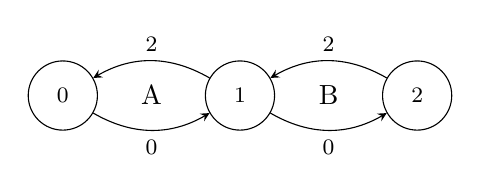
\begin{tikzpicture}[thin, scale=0.75]
        % Nodes
        \draw (-3,0) node(0) [circle,draw,minimum size=25] {\footnotesize \(0\)};
        \draw (0,0)  node(1) [circle,draw,minimum size=25] {\footnotesize \(1\)};
        \draw (3,0)  node(2) [circle,draw,minimum size=25] {\footnotesize \(2\)};

        % Edges
        \path[thin, ->, bend right, >=stealth] (1) edge[above] node {\footnotesize\(2\)} (0);
        \path[thin, ->, bend right, >=stealth] (2) edge[above] node {\footnotesize\(2\)} (1);
        \path[thin, ->, bend right, >=stealth] (0) edge[below] node {\footnotesize\(0\)} (1);
        \path[thin, ->, bend right, >=stealth] (1) edge[below] node {\footnotesize\(0\)} (2);

        \draw (-1.5,0) node[] { A };
        \draw (1.5,0) node[] { B };


      \end{tikzpicture}
      % \caption{\label{fig:three-states} }
    \end{figure}

    \begin{itemize}
    \item Both policies are have an average reward of $1$ (gain-optimal).
    \item But only \(\pol_{A}\) is bias-optimal: $V^{\polopt}(s) - V^{\pol}(s) \geqslant 0$.
    \end{itemize}


    \begin{center}
      \begin{tabular}{rcccc}
        \(s\) & \(V^{\pol_{A}}(s)\) & \(V^{\pol_{B}}(s)\)& \(V_{0.99}^{\pol_{A}}\) & \(V_{0.99}^{\pol_{B}}\)\\
        \toprule
        0 & \(-0.5\) & \(-1.5\) & \(99.4975\)  & \(98.5025\)  \\
        1 & \(0.5\) & \(-0.5\)  & \(100.5025\) & \(99.4975\)  \\
        2 & \(1.5\) & \(0.5\)   & \(101.4975\) & \(100.5025\) \\
        \bottomrule
      \end{tabular}

    \end{center}


  \end{block}
\end{frame}


% % \begin{frame}[t]
% %   \frametitle{Discounted Reinforcement Learning Issues}
% %   \begin{block}{Average Reward}

% %   \end{frame}


%   \begin{frame}[t]

%     \frametitle{Average Reward Example}
%     \begin{block}{Average Reward}


%       \begin{figure}[t!]
%         \centering
%         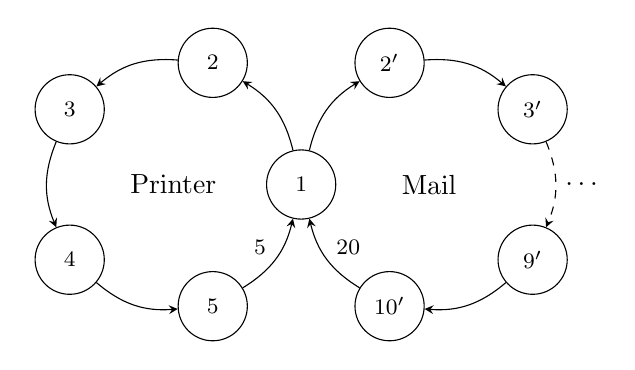
\begin{tikzpicture}[thin, scale=0.65]
  % Nodes
  \foreach \x in {1,...,5}{
    \draw ({cos(\x*72-72)*2.5},{sin(\x*72-72)*2.5}) node(\x) [circle,draw,minimum size=25] {\footnotesize \(\x\)};
  };
  \foreach[evaluate={
    \y=int(\x+5);
  }]  \x in {2,...,3}{
    \draw ({-cos(\x*72-72)*2.5+5},{sin(\x*72-72)*2.5}) node(\y) [circle,draw,minimum size=25]
    {\footnotesize \(\x'\)};
  };
  \foreach [evaluate={
    \y=int(\x+5);
    \z=int(\x+5);
  }] \x in {4,...,5}{
    \draw ({-cos(\x*72-72)*2.5+5},{sin(\x*72-72)*2.5}) node(\z) [circle,draw,minimum size=25]
    {\footnotesize \(\y'\)};
  };

  \newcommand\bend{22.5}
  % Edges
  \path[thin, ->, bend right=\bend, >=stealth] (1) edge[below left] node {\footnotesize\(\)} (2);
  \path[thin, ->, bend right=\bend, >=stealth] (2) edge[above]      node {\footnotesize\(\)} (3);
  \path[thin, ->, bend right=\bend, >=stealth] (3) edge[left ]      node {\footnotesize\(\)} (4);
  \path[thin, ->, bend right=\bend, >=stealth] (4) edge[above]      node {\footnotesize\(\)} (5);
  \path[thin, ->, bend right=\bend, >=stealth] (5) edge[above left] node[yshift=-2] {\footnotesize\(5\)} (1);

  \path[thin, ->, bend left=\bend, >=stealth]         (1)  edge[below right] node {\footnotesize\(\)} (7);
  \path[thin, ->, bend left=\bend, >=stealth]         (7)  edge[above right] node {\footnotesize\(\)} (8);
  \path[thin, ->, dashed, bend left=\bend, >=stealth] (8)  edge[right]       node {\(\ldots\)} (9) ;
  \path[thin, ->, bend left=\bend, >=stealth]         (9)  edge[above]       node {\footnotesize\(\)} (10);
  \path[thin, ->, bend left=\bend, >=stealth]         (10) edge[above right] node[yshift=-2] {\footnotesize\(20\)} (1);

  \draw (0,0) node[] { Printer };
  \draw (5,0) node[] { Mail };

\end{tikzpicture}

%%% Local Variables:
%%% mode: latex
%%% TeX-master: "../paper"
%%% End:


%       \end{figure}
%       \vspace{-0.25cm}
%       \begin{itemize}
%       \item Average reward is \(1\) for the printer- and \(2\) for the mail-loop.\pause
%       \item Only choosing the mail-loop is \alert{gain-optimal}:
%         \begin{align*}
%           \avgrew^{\polopt}(s) - \avgrew^{\pol}(s) \geqslant 0
%         \end{align*}

%       \end{itemize}

%     \end{block}

%   \end{frame}

%   \begin{frame}[t]
%     \frametitle{The Need for Bias Values}

%     \begin{block}{Another example~\footnotemark}

%       \begin{figure}[t!]
%         \centering
%         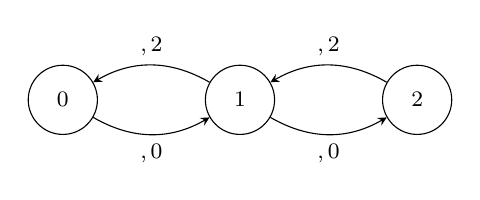
\begin{tikzpicture}[thin, scale=0.75]
  % Nodes
  \draw (-3,0) node(0) [circle,draw,minimum size=25] {\footnotesize \(0\)};
  \draw (0,0)  node(1) [circle,draw,minimum size=25] {\footnotesize \(1\)};
  \draw (3,0)  node(2) [circle,draw,minimum size=25] {\footnotesize \(2\)};

  % Edges
  \path[thin, ->, bend right, >=stealth] (1) edge[above] node {\footnotesize\(\lft,2\)} (0);
  \path[thin, ->, bend right, >=stealth] (2) edge[above] node {\footnotesize\(\lft,2\)} (1);
  \path[thin, ->, bend right, >=stealth] (0) edge[below] node {\footnotesize \(\rght,0\)} (1);
  \path[thin, ->, bend right, >=stealth] (1) edge[below] node {\footnotesize \(\rght,0\)} (2);

  % \draw (-1.5,0) node[] { A };
  % \draw (1.5,0) node[] { B };
\end{tikzpicture}

%%% Local Variables:
%%% mode: latex
%%% TeX-master: "../presentation"
%%% End:



%         \caption{\label{fig:three-states} A task with two different deterministic MDPs, A (going left
%         in 1) and B (going right). Both policies, \(\pol_{A}\) and \(\pol_{B}\) respectively, yield
%         an average reward of 1.}
%       \end{figure}
%     \end{block}
%     \pause
%     \begin{block}{}
%       \centering
%       Therefore, we need more refined seperation criteria.
%     \end{block}


%     \footnotetext{Adapted from
%     \cite{Mahadevan96_AverageRewardReinforcementLearningFoundationsAlgorithmsAndEmpiricalResults}}
%   \end{frame}


%   \begin{frame}[t]
%     \frametitle{Average Reward Reinforcement Learning}

%     \begin{block}{Bias Value $\avgrew^{\pol}(s)$ \footnotemark}

%       The \alert{bias value} is defined as
%       \begin{align*}
%         V^{\pol}(s) = \lim_{N \to \infty}{ \E [ \sum_{t=0}^{N-1}(R_{t}^{\pol}(s) - \avgrew^{\pol} )]}\tcom
%       \end{align*}

%       where again \(R_{t}^{\pol}(s)\) is the reward received at time \(t\), starting in state \(s\) and
%       following policy \(\pol\).
%     \end{block}

%     \footnotetext{\cite{Howard64}}

%     \pause
%     \begin{block}{Note}
%       \begin{itemize}
%       \item $V^{\pol}(s)$ bounded due to the subtraction of the average reward.
%       \item Thus, $V^{\pol}(s)$ is additional rewards when starting in state \(s\).
%       \end{itemize}
%     \end{block}
%   \end{frame}


%   \section{Optimality Criteria Revisited}

%   \begin{frame}[t]
%     \frametitle{More Refined Optimality Criteria}

%     \vspace{-1ex}
%     \begin{block}{Recap}
%       \begin{minipage}[t]{0.08\textwidth}
%         \
%       \end{minipage}
%       \begin{minipage}[t]{0.85\textwidth}

%         \begin{enumerate}
%         \item[\only<1-3>{1.}\only<4->{$n=-1$:}] Gain optimality: Highest average reward.
%         \item[\only<1-3>{2.}\only<5->{$n=0$:}] Bias optimality: Highest bias value, that is collecting rewards as soon as possible.
%         \end{enumerate}
%       \end{minipage}
%     \end{block}\pause

%     \begin{definition}
%       Due to \footnotemark{} a policy \(\polopt\) is \alert{\(n\)-discount-optimal} for
%       \(n=-1,0,1,\ldots\) for all states \(s \in \States\) with discount factor \(\gamma\)
%     %       
%       if and only if
%       \begin{align*}
%         \lim_{\gamma \to 1}(1-\gamma)^{-n}\ (V_{\gamma}^{\polopt}(s) - V_{\gamma}^{\pol}(s)) \geqslant 0 \tpkt
%       \end{align*}
%       \only<3->{If a policy is $\infty$-discount optimal it is called Blackwell-optimal\footnotemark.}

%     \end{definition}

%     \only<1-2>{  \vspace{-1ex} \footcitetext{Veinott69}}
%     \only<3->{  \vspace{-1ex} \footcitetext{Blackwell62}}
%   \end{frame}

%   \section{Discounted and Average Reward Reinforcement Learning}


%   \begin{frame}[t]
%     \frametitle{Laurent Series Expansion of Discounted State Values}

%     \begin{block}{Laurent Series Expansion of Discounted State Values\footnotemark}
%       The Laurent series expansion of $V_{\gamma}^{\pol}(s)$ connected average reward RL and
%       discounted RL:
%       \begin{align*}
%         V_{\gamma}^{\pol}(s) = \frac{\avgrew^{\pol}(s)}{1-\gamma} + V^{\pol}(s) + e_{\gamma}^{\pol}(s)
%       \end{align*}
%     \end{block}
%     \only<1-1>{\footnotetext{\cite{MillerVeinott1969}}}
%     \only<3->{\footnotetext{\cite{MillerVeinott1969}}}

%     \only<2-2>{
%     \begin{block}{Convergence of $e_{\gamma}^{\pol}$ \footnotemark{}}
%       $e_{\gamma}^{\pol}(s)$ consists of infinitely many terms which alternate in its sign, but
%       \vspace{-2ex}
%       \begin{align*}
%         \lim_{\gamma \to 1} e_{\gamma}^{\pol}(s) = 0
%       \end{align*}
%     \end{block}
%     \footnotetext{\cite{Puterman94}}
%   }
%     \only<3->{
%     \begin{block}{Note \only<3-3>{1}\only<4->{2}}
%       \begin{enumerate}
%         \only<3-3>{\item First term converges to infinity as \(\gamma\) increases.}
%         \only<4->{
%       \item First term: maximise average reward (gain-optimality)
%       \item Second term: maximise bias value (bias-optimality)
%       \item Third term: collect rewards as soon and in as little steps as possible
%       }
%       \end{enumerate}

%     \end{block}
%   }


%   \end{frame}


%   \begin{frame}[t]
%     \frametitle{Recursive Form of the Laurent Series Expansion}
%     \begin{block}{Reformulation in Recursive Scheme\footnotemark}
%       Let \(n=-1,0,\ldots\) denote the coefficients of the the Laurent series
%       expansion, then:\vspace{-2ex}
%       \begin{align*}
%         \avgrew^{\pol}(s) - E[\avgrew^{\pol}(s)] & = 0 & & \text{for } n = -1 \\
%         \avgrew^{\pol}(s) + V^{\pol}(s) - E[V^{\pol}(s)] & = r(s,a) && \text{for } n = 0 \\
%         W^{\pol}_{n-1}(s) + W^{\pol}_{n}(s) - E[W^{\pol}_{n}(s)] & = 0 && \text{for } n \geqslant 1,\\
%         & && \text{where } W_{0}^{\pol}(s) = V^{\pol}(s)
%       \end{align*}
%     \end{block}

%     \only<1-1>{\footnotetext{\cite{MillerVeinott1969} and \cite[p.346]{Puterman94}}}
%     \only<3->{\footnotetext{\cite{MillerVeinott1969} and \cite[p.346]{Puterman94}}}

%     \only<2-2>{
%     \begin{block}{}
%       If \(n=-1,0,\ldots,M\) constraints are satisfying the above conditions for all states \(s\),
%       then only \(\avgrew^{\pol}(s), V^{\pol}(s), W^{\pol}_{1}, \ldots, W^{\pol}_{M-1}\) are
%       unique.\footnotemark
%     \end{block}
%     \footnotetext{\cite[p.346]{Puterman94}}
%   }

%     \only<3->{
%     \begin{block}{Strategy}
%       Solve with above for $n=-1$, $n=0$ and $n=1$, and for $e_{\gamma}^{\pol}(s)$ $\ldots$
%     \end{block}
%   }


%   \end{frame}

%   \begin{frame}[t]
%     \frametitle{}
%     \begin{block}{Idea Sketch}

%       \begin{figure}
%         \centering
%         \begin{tikzpicture}[scale=6]
%           \draw[->] (0,0) -- (1.0,0) node[right] {$\gamma$};
%           \draw[->] (0,0) -- (0,0.8) node[above] {$\mathbb{R}$};
%           \draw[scale=1,domain=0.001:0.85,smooth,variable=\x,blue] plot ({\x},{0.1/(1-\x)+0.2});
%           \draw[scale=1,domain=0.001:0.865,smooth,variable=\x,red] plot ({\x},{0.1/(1-\x)+0.2-0.2*(1-\x)^0.5});

%         %           Labels
%           \draw[blue] (0.55,0.64) node () {$\frac{\avgrew^{\pol}(s)}{1-\gamma} + V^{\pol}(s)$};
%           \draw[red] (0.9,0.58) node () {$V_{\gamma}^{\pol}(s)$};
%           \draw (-0.015,0.3) -- (0.015,0.3);
%           \draw (-0.2, 0.3) node[align=left] () {$\avgrew^{\pol}(s) + V^{\pol}(s)$};

%           \draw (-0.015,0.1) -- (0.015,0.1);
%           \draw (-0.111, 0.1) node[] () {$R^{\pol}(s)$};

%           \draw (0.9,-0.015) -- (0.9,0.015) node[below, yshift=-0.2cm] () {$1$};
%           \draw (0.75,-0.015) -- (0.75,0.015) node[below, yshift=-0.2cm] () {$\gamma_{1}$};
%           \draw (0.20,-0.015) -- (0.20,0.015) node[below, yshift=-0.2cm] () {$\gamma_{0}$};

%           \draw (0.5,0.4) -- (0.5,0.258578644) node[midway,left, yshift=-0.2cm] () {$e_{\gamma}^{\pol}(s)$};

%           \draw (0.2,0.146114562) -- (0.75,0.146114562) node[midway, below] () {$\gamma_{1}-\gamma_{0}$};
%           \draw (0.75,0.146114562) -- (0.75,0.5) node[midway,right] () {$V_{\gamma_{1}}^{\pol}(s)-V_{\gamma_{0}}^{\pol}(s)$};


%         \end{tikzpicture}
%       %         \caption{}
%         \label{fig:e}
%       \end{figure}
%       Infer the slope of the error term with $\gamma_{1} > \gamma_{0} \geqslant 0.5$ and the difference
%       of \(V_{\gamma_{1}}^{\pol}(s)\) and \(V_{\gamma_{0}}^{\pol}(s)\).


%     %       \begin{align*}
%     %         \avgrew^{\pol}(s) - E[\avgrew^{\pol}(s)] & = 0 \\
%     %         \avgrew^{\pol}(s) + V^{\pol}(s) - E[V^{\pol}(s)] & = r(s,a) \\
%     %         V^{\pol} + W^{\pol}_{1}(s) - E[W^{\pol}_{1}(s)] & = 0
%     %       \end{align*}
%     \end{block}


%   \end{frame}


%   \begin{frame}[t]
%     \frametitle{Blackwell-Optimal Reinforcement Learning}

%     \begin{block}{Theorem}
%       \label{thm:minmax}
%       If \(\avgrew^{\pol}(s) \geqslant 0\) and for \(\gamma\)-values \(\gamma_{0}, \gamma_{1}\) with
%       \(0.5 \leqslant \gamma_{0} < \gamma_{1} < 1\) a \alert{Blackwell-optimal} agent chooses the
%       action \(s'\) that maximises the expected discounted state value difference
%       \(\Delta V_{\gamma}^{\pol}(s') = V_{\gamma_{1}}^{\pol}(s') - V_{\gamma_{0}}^{\pol}(s')\) of the
%       set of \(0\)-discount-optimal actions available and for which
%       \begin{itemize}
%       \item \(\frac{\avgrew}{1-\gamma_{0}} + V^{\pol}(s') < V_{\gamma_{0}}^{\pol}(s')\) holds
%         (converging from above), or if
%         no such actions exists, then for which
%       \item \(\frac{\avgrew}{1-\gamma_{0}} + V^{\pol}(s') \geqslant V_{\gamma_{0}}^{\pol}(s')\) hold
%         (converging from below).
%       \end{itemize}
%     \end{block}
%   \end{frame}


%   \begin{frame}[t]
%     \begin{block}{Algorithm (Part 1)}

%       \footnotesize
%       \begin{algorithmic}[1]
%         \State{}Initialize \While{the stopping criterion is not fulfilled}
%         \State{}\begin{minipage}[t]{0.9\textwidth} With probability \(p_{exp}\) choose a random action
%           and probability \(1-p_{exp}\) one that maximizes
%           \(\lex(\avgrew^{\pol}(s,a),\V^{\pol}(s,a),\Delta V^\pol_\gamma(s,a))\) at the current state
%           \(s\) where \(\Delta V^\pol_\gamma(s,a) = V^\pol_{\gamma_1}(s,a) - V^\pol_{\gamma_0}(s,a)\)
%           for all actions for which
%           \(\frac{\avgrew^{\pol}(s,a)}{1-\gamma_{0}} + \V^{\pol}(s,a) < V^\pol_{\gamma_0}(s,a)\) holds or if no
%           such actions exists, from all actions.
%         \end{minipage}
%         \State{}Carry out action \(a\), observe reward \(r\) and resulting state \(s'\)
%       %         \State{}If non-random action update values
%         \State{}Update values using exponential smoothing
%         \begin{align*}
%           \avgrew^{\pol}(s,a)  & \gets (1-\alpha) \avgrew^{\pol}(s,a) + \alpha (r + \max_{a}\V^{\pol}(s',a) - \V^{\pol}(s,a))     \\
%           \V^{\pol}(s,a)        & \gets (1-\beta) \V^{\pol}(s,a) + \beta (r - \avgrew^{\pol}(s,a) + \max_{a} \V^{\pol}(s',a))     \\
%           W^{\pol}(s,a)        & \gets (1-\delta) W^{\pol}(s,a) + \delta (-\V^{\pol}(s,a) + \max_{a} W^{\pol}(s',a))              \\
%           \Psi_{V}(s,a) & \gets (1-\gamma) \Psi_{V}(s,a) + \gamma (r - \avgrew(s,a) - V(s,a) + \max_{a} V(s',a))\\
%           \Psi_{W}(s,a) & \gets (1-\gamma) \Psi_{W}(s,a) + \gamma (- V^{\pol}(s,a) - W^{\pol}(s,a) + \max_{a} W^{\pol}(s',a))
%         \end{align*}
%         \algstore{bkbreak}
%       \end{algorithmic}
%     \end{block}


%   \end{frame}

%   \begin{frame}[t]
%     \begin{block}{Algorithm (Part 2)}

%       \footnotesize
%       \begin{algorithmic}[1]
%         \algrestore{bkbreak}
%         \State{}Update discounted state-values
%         \begin{align*}
%           V^\pol_{\gamma_0}(s,a)    & \gets (1-\gamma) V^\pol_{\gamma_0}(s,a) + \gamma (r + \gamma_{0} \max_{a} V^\pol_{\gamma_0}(s',a)) \\
%           V^\pol_{\gamma_1}(s,a)    & \gets (1-\gamma) V^\pol_{\gamma_1}(s,a) + \gamma (r + \gamma_{1} \max_{a} V^\pol_{\gamma_1}(s',a))
%         \end{align*}
%         \If{If non-random action was chosen}
%         \If{t is even}
%         \State{\( \qquad  \V^{\pol}(s,a)  \gets \V^{\pol}(s,a) + \xi \cdot \Psi_{V}(s,a)\)}
%         \Else
%         \State{\( \qquad  \V^{\pol}(s,a)  \gets \V^{\pol}(s,a) + \xi \cdot \Psi_{W}(s,a)\)}
%         \EndIf
%         \EndIf
%         \State{} Set \(s \gets s'\), \(t \gets t+1\) and possibly update parameters
%         \EndWhile{}
%       \end{algorithmic}
%     \end{block}

%     \begin{block}{Note}
%       \begin{itemize}
%       \item Lines $7-11$ enforce the correct state values (close loop of recursive scheme) and are
%         crucial for finding correct values. No other algorithm incorporated them yet.
%       \item Therefore, no reference state is needed as in other algorithms.
%       \end{itemize}
%     \end{block}
%   \end{frame}

%   \begin{frame}[t]
%     \frametitle{Refinements}

%     \begin{block}{Refinements}
%       \begin{itemize}
%       \item We assume a unichain MDP and thus use a scalar value for the average reward.
%       \item The average reward may also be observed using a moving average.
%       \item We keep track of the average reward over time and prevent its decrease.
%       \item We stop learning from random actions once the exploration rate is below a certain level,
%         as in case of random actions $\Psi_{\cdot}(s,a) \neq 0$.
%       \end{itemize}

%     \end{block}
%   \end{frame}

%   \begin{frame}[t]
%     \frametitle{Proof of Concept}

%     \begin{block}{Proof of Concept}
%       The previous examples can be solved by inferring correct state values by the algorithm in both
%       \begin{itemize}
%       \item the model-based, and
%       \item the model-free case.
%       \end{itemize}
%     \end{block}
%     \pause
%     \begin{block}{Current Main Downsides/Challanges}
%       \begin{itemize}
%       \item Number of learning steps needed increased by factor $3-10$
%       \item Stability not yet perfect: While solving the policy may jump from good to bad solutions
%         and vice versa various times
%       \end{itemize}


%     \end{block}


%   \end{frame}


% % %%%%%%%%%%%%%%%%%%%%%%%%%%%%%%   


%   \section{Order Release with Average Reward Reinforcement Learning}


%   \begin{frame}[t]
%     \frametitle{Hypothetical Flow Shop}

%   %     \begin{block}{Problems in Operation Research Domain}
%   %       \begin{itemize}
%   %       \item Periodic and discrete decisions
%   %       \item Maximizing profits
%   %       \item High degree of complexity
%   %       \end{itemize}
%   %     \end{block}

%     \vspace{-1.5ex}
%     \begin{block}{}

%       \hspace*{-1.4ex}\begin{tikzpicture}[queue/.style={regular polygon,regular polygon sides=4,inner sep=0.075cm},scale=0.8]

  \draw (-3.5,0) node[] {$\ldots$};
  \draw (-4.1,-1.75) node[] {\scriptsize Due Date:};

  \draw (-3.0,-1.5) -- (-3.0,1.5)
        (-2.5,1.5)  -- (-2.5,-1.5)
        (-2.5,-1.5) -- (-3.0,-1.5);
  \draw (-2.75,-1.75) node[] {\tiny $t+3$};

  \draw (-2.5,-1.5) -- (-2.5,1.5)
        (-2,1.5)  -- (-2,-1.5)
        (-2,-1.5) -- (-2.5,-1.5);
  \draw (-2.25,-2) node[] {\tiny $t+2$};
  \draw (-2 ,-1.5) -- (-2,1.5)
        (-1.5,1.5)  -- (-1.5,-1.5)
        (-1.5,-1.5) -- (-2,-1.5);
  \draw (-1.75,-1.75) node[] {\tiny $t+1$};

  \draw (-1.5,0.0) node[] (OP) {};
  % \draw [decorate,decoration={brace,amplitude=5pt},xshift=-2pt,yshift=0pt] (-1.0,-2.25) -- (-3.75,-2.25)     node [black,midway,yshift=-0.4cm] {\scriOrder Pool};
  % \draw [decorate,decoration={brace,amplitude=5pt},xshift=-2pt,yshift=0pt] (5.0,-2.25) -- (-.75,-2.25)  node [black,midway,yshift=-0.4cm] {Production System};
  % \draw [decorate,decoration={brace,amplitude=5pt},xshift=-2pt,yshift=0pt] (7,-2.25) -- (5.25,-2.25) node [black,midway,yshift=-0.4cm] {Inventory};

  % \draw (-1.75,-1.3) node[circle,inner sep=1pt,minimum size=0.2cm,draw] {$\scriptscriptstyle 1$};
  % \draw (-1.75,-1.0) node[circle,inner sep=1pt,minimum size=0.2cm,draw] {$\scriptscriptstyle 1$};
  % \draw (-1.75,-0.7) node[circle,inner sep=1pt,minimum size=0.2cm,draw] {$\scriptscriptstyle 2$};
  % \draw (-1.75,-0.4) node[circle,inner sep=1pt,minimum size=0.2cm,draw] {$\scriptscriptstyle 2$};
  % \draw (-1.75,-0.1) node[circle,inner sep=1pt,minimum size=0.2cm,draw] {$\scriptscriptstyle 3$};
  % \draw (-1.75, 0.2) node[circle,inner sep=1pt,minimum size=0.2cm,draw] {$\scriptscriptstyle 3$};
  % \draw (-1.75, 0.5) node[circle,inner sep=1pt,minimum size=0.2cm,draw] {$\scriptscriptstyle 4$};
  % \draw (-1.75, 0.8) node[circle,inner sep=1pt,minimum size=0.2cm,draw] {$\scriptscriptstyle 4$};
  % \draw (-1.75, 1.1) node[circle,inner sep=1pt,minimum size=0.2cm,draw] {$\scriptscriptstyle 6$};
  % \draw (-1.75, 1.4) node[circle,inner sep=1pt,minimum size=0.2cm,draw] {$\scriptscriptstyle 6$};
  % \draw (-1.75, 1.7) node[circle,inner sep=1pt,minimum size=0.2cm,draw] {$\scriptscriptstyle 6$};

  \draw (-2.25,-1.3) node[circle,inner sep=1pt,minimum size=0.2cm,draw] {$  \scriptscriptstyle 1$};
  \draw (-2.25,-0.95) node[circle,inner sep=1pt,minimum size=0.2cm,draw] {$ \scriptscriptstyle 2$};
  \draw (-2.25,-0.6) node[circle,inner sep=1pt,minimum size=0.2cm,draw] {$  \scriptscriptstyle 1$};
  \draw (-2.25,-0.25) node[circle,inner sep=1pt,minimum size=0.2cm,draw] {$ \scriptscriptstyle 1$};

  \draw (-2.75,-1.3) node[circle,inner sep=1pt,minimum size=0.2cm,draw] {$  \scriptscriptstyle 1$};
  \draw (-2.75,-0.95) node[circle,inner sep=1pt,minimum size=0.2cm,draw] {$ \scriptscriptstyle 1$};
  \draw (-2.75,-0.6) node[circle,inner sep=1pt,minimum size=0.2cm,draw] {$  \scriptscriptstyle 2$};
  \draw (-2.75,-0.25) node[circle,inner sep=1pt,minimum size=0.2cm,draw] {$ \scriptscriptstyle 2$};
  \draw (-2.75, 0.1) node[circle,inner sep=1pt,minimum size=0.2cm,draw] {$  \scriptscriptstyle 2$};
  \draw (-2.75, 0.45) node[circle,inner sep=1pt,minimum size=0.2cm,draw] {$ \scriptscriptstyle 1$};
  \draw (-2.75, 0.8) node[circle,inner sep=1pt,minimum size=0.2cm,draw] {$  \scriptscriptstyle 2$};

  \draw (0.7,0)    node[minimum size=1cm,draw,align=center] (M1) {WC1\\[-1ex]{\tiny $\Unif(70,130)$}};
  \draw (3.45,0.75)   node[minimum size=1cm,draw,align=center] (M2) {WC2\\[-1ex]{\tiny  $\Unif(130,170)$}};
  \draw (3.45,-0.75)  node[minimum size=1cm,draw,align=center] (M3) {WC3\\[-1ex]{\tiny $\Unif(180,200)$}};
  % \draw (6,1.5)    node[minimum size=1cm,draw,align=center] (M4) {M4\\[-1ex]{\tiny $\Exp(210)$ or}\\[-1ex]{\tiny $\Unif(50,370)$}};
  % \draw (6,0)      node[minimum size=1cm,draw,align=center] (M5) {M5\\[-1ex]{\tiny $\Exp(285)$ or}\\[-1ex]{\tiny $\Unif(200,370)$}};
  % \draw (6,-1.5)   node[minimum size=1cm,draw,align=center] (M6) {M6\\[-1ex]{\tiny $\Exp(215)$ or}\\[-1ex]{\tiny $\Unif(110,320)$}};
  \draw (6,0)      node[minimum size=1cm,draw,align=center,fill] (\fgi{}) {\color{white} \fgi{}};

  \draw (M1.west) node[draw,queue,minimum size=0.05cm,fill,xshift=-0.075cm] (Q1) {};
  \draw (M2.west) node[draw,queue,minimum size=0.05cm,fill,xshift=-0.075cm] (Q2) {};
  \draw (M3.west) node[draw,queue,minimum size=0.05cm,fill,xshift=-0.075cm] (Q3) {};
  % \draw (M4.west) node[draw,queue,minimum size=0.05cm,fill,xshift=-0.075cm] (Q4) {};
  % \draw (M5.west) node[draw,queue,minimum size=0.05cm,fill,xshift=-0.075cm] (Q5) {};
  % \draw (M6.west) node[draw,queue,minimum size=0.01cm,fill,xshift=-0.075cm] (Q6) {};

  \draw (8.5, 1) node[] (CustomerTop) {\Huge \Gentsroom};
  \draw (8, 0.5) node[] {\Huge \Ladiesroom};
  \draw (8.5, 0) node[] (Customer) {\Huge \Gentsroom};
  \draw (8,-0.5) node[] {\Huge \Ladiesroom};
  \draw (8.5,-1) node[] {\Huge \Gentsroom};

  % Paths
  \path (OP.center) edge[->, bend left=10]
  node[xshift=0.088cm,yshift=0.12cm,align=center] {\scriptsize \alert{Order} \\[-1ex] \scriptsize
    \alert{Release} \\[1.05ex] \scriptsize % \alert{via LT}
  } (Q1);

  
  \path (M1) edge[->, bend left=10, above]                 node[xshift=-0.1cm,yshift=-0.05cm] {$\scriptstyle % \text{P}1
    $} (Q2);
  \path (M1) edge[->, bend right=10,above]                 node[xshift=0.1cm,yshift=-0.05cm] {$\scriptstyle % \text{P}2
    $} (Q3);
  % \path (M2) edge[->, bend left=10,above,near start ]      node {$\scriptstyle 1$}     (Q4);
  % \path (M2) edge[->, bend left=10,above,near start ]      node {$\scriptstyle 2$}     (Q5);
  % \path (M2) edge[->, bend left=10,above,near start ]      node[xshift=0.06cm,yshift=-0.1cm] {$\scriptstyle 3$}     (Q6);
  % \path (M3) edge[->, bend right=10,above,very near start] node[xshift=0.20cm,yshift=-0.15cm] {$\scriptstyle 4$}     (Q4);
  % \path (M3) edge[->, bend right=10,above,very near start]      node[yshift=-0.075cm] {$\scriptstyle 5$}     (Q5);
  % \path (M3) edge[->, bend right=10,above,near start]      node {$\scriptstyle 6$}     (Q6);
  % \path (M4) edge[->, bend left=10,above,near start]       node[xshift=0.1cm] {$\scriptstyle 1,4$} (\fgi{});
  \path (M2) edge[->, bend left=10,above,near start]       node[xshift=0.1cm, yshift=-0.07cm] {$\scriptstyle % \text{P}1
    $} (\fgi{});
  \path (M3) edge[->, bend right=10,above,near start]      node[xshift=0.07cm,yshift=0.07cm] {$\scriptstyle % \text{P}2
    $} (\fgi{});

  \path (\fgi{}) edge[->,near start] node[xshift=0.1cm,align=left] {\tiny Not \\[-1ex]
    \tiny before \\[-0.5ex] \tiny due \\[-1ex] \tiny date}    (Customer);

  \path (CustomerTop) edge[densely dashed] (8.5,2.8);
  \path (8.5,2.8) edge[densely dashed,midway,align=center] node[yshift=0.0cm] {\scriptsize Customer places
    an order which initiates the process\\ {\tiny Distribution of incoming orders:
      $\Unif(3,15)$ % or $\Exp(105)$ or $\Unif(65, 145)$
    }
  } (-4.5, 2.8);
  \path (-4.5,2.8) edge[densely dashed] (-4.5,0);
  \path (-4.5,0) edge[->,densely dashed] (-4.0,0);


\end{tikzpicture}


%%% Local Variables:
%%% mode: latex
%%% TeX-master: "../presentation"
%%% End:


%       \begin{itemize}
%       \item Make-to-order flow-shop (bottleneck util. 90\%) with FCFS dispatching
%       \item Holding costs, WIP costs and Backorder costs
%       \end{itemize}

%     \end{block}

%   \end{frame}

%   \begin{frame}[t]
%     \frametitle{Markov Decision Process I}

%     \begin{block}{Action Space: Setting the Lead Times per product type (LT$_{p}$)}
%       \begin{itemize}
%       \item Relative change to last period: $-1, 0, +1$ for each product $p$ \pause
%       \item Order $i$ of product $p$ is released at period $t$ according to following formula.
%         \[
%           \text{Release Order}_{i} =
%           \begin{cases}
%             \text{Yes} & \qquad \text{if: } \text{Due Date}_{i} - LT_{p} \leqslant t\\
%             \text{No} &  \qquad \text{otherwise}
%           \end{cases}
%         \]
%       \end{itemize}
%     \end{block}

%   \end{frame}

%   \begin{frame}[t]
%     \frametitle{Markov Decision Process II}

%     \begin{block}{State Space for each product $p$}
%       \begin{itemize}
%       \item Lead Time of preceding period
%       \item Number of orders in the order pool $^{\star}$
%       \item Number of orders in each queue
%       \item Number of orders in the finished goods inventory $^{\star}$
%       \item Number of orders shipped in the last period $^{\star}$
%       \end{itemize}
%       \begin{minipage}[t]{\textwidth}
%         \centering
%         {\footnotesize $^{\star}$ Grouped into time buckets by periods until due.}

%       \end{minipage}

%     \end{block}

%   \end{frame}

%   \begin{frame}[t]
%     \frametitle{Markov Decision Process III}

%     \begin{block}{Reward}
%       \begin{itemize}
%       \item Accumulated costs $\mathsf{C}$ at the end of period given by
%         \begin{itemize}
%         \item Backorders (overdue orders): \\$20$ \euro{} per order and period \pause
%         \item Orders in the production system (WIP): \\$3$ \euro{} per order and period \pause
%         \item Orders in the finished goods inventory: \\$10$ \euro{} per order and period
%         \end{itemize}\pause
%       \item Reward Function: $50 - 0.5 \cdot \mathsf{C}$, then divided by normalising parameter and
%         clipped to $[-1,1]$
%       \end{itemize}
%     \end{block}


%   \end{frame}


% %   \begin{frame}
% %     \frametitle{Hypothetical Flow Shop II}

% %     \begin{block}{Production System}

% %       Bildl vom PS mit BAZ und Products $p$

% %     \end{block}


% %   \end{frame}

% %   \section{Reinforcement Learning Algorithm}
% %   \label{sec:Reinforcement_Learning_Algorithm}


% %   \begin{frame}[t]
% %     \frametitle{Markov Decision Process}

% %     \begin{block}{Markov Decision Process (MDP)}
% %       \begin{itemize}
% %       \item MDP is unichain
% %       \item Action space and state space are discrete
% %       \end{itemize}
% %     \end{block}
% %     \pause

% %     \begin{block}{Action Space: Setting the Lead Times (LT$_{p}$)}
% %       \begin{itemize}
% %       \item Relative change to last period: $-1, 0, +1$ for each product $p$ \pause
% %       \item Order $i$ of product $p$ is released at period $t$ according to following formula.
% %         \[
% %           \text{Release Order}_{i} =
% %           \begin{cases}
% %             \text{Yes} & \qquad \text{if: } \text{Due Date}_{i} - LT_{p} \leqslant t\\
% %             \text{No} &  \qquad \text{otherwise}
% %           \end{cases}
% %         \]
% %       \end{itemize}


% %     \end{block}

% %   \end{frame}


% %   \begin{frame}[t]
% %     \frametitle{Markov Decision Process II}

% %     \begin{block}{State Space for each product $p$}
% %       \begin{itemize}
% %       \item Lead Time of preceding period
% %       \item Number of orders in the order pool $^{\star}$
% %       \item Number of orders in each queue
% %       \item Number of orders in the finished goods inventory $^{\star}$
% %       \item Number of orders shipped in the last period $^{\star}$
% %       \end{itemize}
% %       \begin{minipage}[t]{\textwidth}
% %         \centering
% %         {\footnotesize $^{\star}$ Grouped into time buckets by periods until due.}

% %       \end{minipage}

% %     \end{block}

% %   \end{frame}
% %   \begin{frame}[t]
% %     \frametitle{Markov Decision Process III}

% %     \begin{block}{Reward}
% %       \begin{itemize}
% %       \item Accumulated costs at the end of period given by
% %         \begin{itemize}
% %         \item Backorders (overdue orders): \\$20$ \euro{} per order and period \pause
% %         \item Orders in the production system (WIP): \\$3$ \euro{} per order and period \pause
% %         \item Orders in the finished goods inventory: \\$10$ \euro{} per order and period
% %         \end{itemize}\pause
% %       \item Divided by normalising parameter $\eta$ and clipped to $[-0.5,0.5]$
% %       \end{itemize}

% %     \end{block}


% %   \end{frame}


% %   \begin{frame}[t]
% %     \frametitle{Adapted Reinforcement Learning Algorithm}

% %     \begin{block}{Adapted Reinforcement Learning Algorithm}
% %       Actor-critic algorithm similar to A3C\footnotemark, but with \pause
% %       \begin{itemize}
% %       \item Experience Replay, \pause
% %       \item State-Action values instead of state values only, \pause
% %       \item Forking the current state to explore different actions, \pause
% %       \item May use average reward reinforcement learning, and \pause
% %       \item Softly updating target networks $\netPTarget$,
% %         $\netQTarget$ as in~\cite{lillicrap2015continuous}:
% %         \begin{align*}
% %           \netQTarget(s,a) & \gets \tau \cdot \netQTarget(s,a) + (1-\tau) \cdot  \netQ(s,a)\\
% %           \netPTarget(s,a) & \gets \tau \cdot \netPTarget(s,a) + (1-\tau) \cdot  \netP(s,a)
% %         \end{align*}
% %         All workers operate on the worker networks $\netP$ and $\netQ$.
% %       \end{itemize}
% %       \footnotetext{\cite{mnih2016asynchronous}}

% %     \end{block}
% %   \end{frame}


% %   \begin{frame}[t]
% %   %     \frametitle{Adapted Reinforcement Learning Algorithm II}
% %     \begin{block}{Adapted Reinforcement Learning Algorithm (Simplified)}

% %       \begin{algorithmic}[1]
% %         \footnotesize
% %         \algrenewcommand\algorithmicindent{1.0em}%
% %         \State{\only<1-1>{\alert}{Perform initialization; Choose algorithm by setting $\mathsf{alg} \in \{0,1\}$ }}
% %         \Repeat~(for each step and worker $w_{1},\ldots,w_{W}$)
% %         \State{\only<2-2>{\alert}{Take action $a_{t}$ accord. to
% %         $\pi(a_{t} \mid s_{t}; \theta^{T}_{\pi})$, observe reward $r_{t}$ and state $s_{t+1}$}}
% %         \State{\only<3-3>{\alert}{Forking: With probability $p_{f}$ copy state $s_{t}$ and explore different action}}
% %         \State{\only<4-4>{\alert}{Store all experiences $(s_{t},a_{t},r_{t},s_{t+1})$ to the replay memory $\mathcal{E}$}}
% %         \State{\only<5-5>{\alert}{Avg. reward: $\rho \gets (1-\alpha) \rho + \alpha [r_{t} + \max_{a}Q(s_{t+1},a) -
% %         \max_{a}Q(s_{t},a)]$}}
% %         \State{\only<6-6>{\alert}{Randomly choose a subset $\mathcal{E}_{t} \subset \mathcal{E}$ of size $n$}}
% %         \State{{Reset gradients $d\netQ \gets 0$, $d\netP \gets 0$}}
% %         \Repeat~(for each experience instance $(s_{e},a_{e},r_{e},s_{e+1}) \in \mathcal{E}_{t}$)
% %         \State{\only<7-7>{\alert}{Save target value $\Qtarget \gets r_{e} + \gamma \cdot \max_{a}Q(s_{e+1},a;
% %         \theta_{Q}^{T}) - (1-\mathsf{alg}) \rho$}}
% %         \State{\only<8-8>{\alert}{Accumulate gradients: $d\theta_{Q} \gets d\theta_{Q} + {\partial(\Qtarget -
% %         Q(s_{e},a_{e}; \theta_{Q}))^{2}}/{\partial{\theta_{Q}}}$}}
% %         \State{\only<8-8>{\alert}{Accumulate gradients:} \\
% %         \only<8-8>{\alert}{\hspace{1.4cm}$d\theta_{\pi} \gets d\theta_{\pi} + \frac{\partial \log \pi(a_{e}\mid s_{e};
% %         \netP) (\Qtarget - \mathsf{alg} \avg_{a}Q(s_{e},a;\theta_{Q}))}{\partial{\theta_{\pi}}}$}}
% %         \Until{all experiences in $\mathcal{E}_{t}$ processed}
% %         \State{\only<9-9>{\alert}{[Synchronized] Update worker networks $\netQ$, $\netP$ using $d\netQ$ and
% %         $d\netP$}}
% %         \State{\only<10-10>{\alert}{[Only if $w_{1}$] Softly update target networks}}
% %         \State{{$t \gets t + 1$}}
% %         \Until{$t \geqslant T$}
% %       \end{algorithmic}
% %     \end{block}

% %   \end{frame}


% %   \begin{frame}[t]
% %     \frametitle{Variants}
% %     \begin{block}{Variants and Two Delays}
% %       \begin{itemize}
% %       \item $\ActShipped{}$: Costs occurring at end of period.
% %         \begin{itemize}
% %         \item Delayed rewards for traversing to good state (standard in RL)
% %         \item Delay until action can be seen in reward due to production
% %         \end{itemize} \pause
% %       \item $\ActShippedAvg{}$: $\ActShipped{}$ with averaging reward per order\pause
% %       \item $\ActShippedAvgRL{}$: $\ActShipped{}$ but using average reinforcement learning. Thus
% %         $\mathsf{alg}=1$.\pause
% %       \item $\ActRelOrds{}$: Keeps track of \only<5->{\alert}{released orders} until reward for taken action is
% %         known.\pause
% %       \item $\ActOrdPool{}$: Keeps track of \alert{current orders in the order pool} until reward for
% %         taken action is known.
% %       \end{itemize}
% %     \end{block}
% %   \end{frame}

% %   \begin{frame}[t]
% %     \frametitle{External Benchmark}

% %   %     \begin{block}{Neural Network Setup (Manually optimized)}
% %   %       \begin{itemize}
% %   %       \item Two three layer fully-connected networks
% %   %       \item Both use 41-ReLU-89-ReLU-20-ReLU-9, with output activations being
% %   %         \begin{itemize}
% %   %         \item Softmax (normalized exponential) -- action probabilities
% %   %         \item Tanh (hyperbolic tangent) -- expected discounted/avg reward
% %   %         \end{itemize}
% %   %       \end{itemize}
% %   %     \end{block}

% %     \begin{block}{External Benchmark}
% %       Backward infinite loading (\BIL{})~\footnotemark:
% %       \begin{align*}
% %       %         \text{Release period}_{\text{Order}} = \text{Due Date}_{\text{Order}} - LT_{p}
% %         \text{Release period} = \text{Due Date} - LT
% %       \end{align*}
% %       where lead time $LT$ is static and predetermined.
% %     \end{block}
% %     \footnotetext{\cite{Ackerman1963}}


% %   \end{frame}

%   \section{Results}
%   \label{sec:Results}


%   \begin{frame}[t]
%     \frametitle{Results}
%     \definecolor{lightgray}{rgb}{0.83, 0.83, 0.83}
%     \begin{block}{Experimental Results}

%       \begin{table}[t!]
%         \footnotesize
%         \centering
%         \def\arraystretch{1.2}          %  1 is the default, change whatever you need
%         \setlength\tabcolsep{4pt}
%         \begin{tabular}{|l||c|c|c|c|c|c|c|c|}
%         %           BEGIN RECEIVE ORGTBL res2
%           \hline
%           Algorithm/KPI & SUM & BOC & FGIC & WIPC & % \%SL &
%           TARD & \(\sigma\)TARD \\
%           \hline
%         %           Evaluation 1 \\
%         %           \ActShipped    & 1777.74 & 1322.04 & 94.49 & 361.20       & 2.24 & 1.52 \\
%           \ActOrdPool$_{\text{Paper}}$    & 1593.03 & 1318.65 &14.01 &260.36         & 2.11 & 1.42 \\
%           \ActOrdPool$_{\text{Current}}$    & 1393.44 & 427.34  & 703.495 & 262.60        & 2.06 & 1.39 \\
%         %           \ActShippedDQN & 1940.62 & 1570.40 &6.30 &363.92          & 2.35 & 1.59 \\
%         %           \ActOrdPoolDQN & 1618.88 & 1306.20 & 40.68& 272.00        & 2.08 & 1.38 \\
%           \BILOne        & 1736.98 & 1510.42  &  0.00  & 226.56     & 2.04 & 1.26 \\
%           \BILTwo        & 1081.79 & 769.86 & 86.89   & 225.03      & 1.87 & 1.18 \\
%           \BILThree      &  \textbf{922.36} & 362.59 &  334.47  & 225.30     & 1.74 & 1.07 \\
%           \BILFour       & 1062.68 & 155.72  & 681.03   & 225.93    & 1.63 & 0.99 \\
%           \BILFive       & 1380.04 & 65.45  & 1088.94    & 225.64   & 1.67 & 1.02 \\
%           \BILSix        & 1777.77 & 25.04 &  1529.77  & 222.96     & 1.61 & 0.85 \\
%         %           \imre          & 2209.97 & 12.08 &1974.72 & 223.16        & 1.58 & 0.63 \\
%           \hline
%         %           END RECEIVE ORGTBL res2
%         \end{tabular}
%       %         \egroup

%       %         \caption{\label{tbl:res}Evaluation results where the monetary units are in \(k\)-values.}

%       %       \end{figure}
%     \end{table}


%     \begin{minipage}[t]{\textwidth}
%       \vspace{-0.5em} \centering {\footnotesize Evaluation results for sum of costs
%       (SUM), backorder costs (BOC), finished goods inventory costs (FGIC), and work in
%       process costs (WIPC) in $10^{3}$ monetary units.}
%     \end{minipage}


%   \end{block}


% \end{frame}

% \section{Future Work}

% \begin{frame}[t]
%   \frametitle{Future Work}
%   %   \begin{block}{Future Work}
%   %     \begin{itemize}
%   %     \item
%   %     \item Forking: decreased learning time, less divergence issues
%   %     \item Representation of rewards has major influence on achievable performance (two delays)
%   %     %     \item Adds to the growing body of evidence that ML can contribute positively to a company's
%   %     %       performance
%   %     \end{itemize}


%   %   \end{block} \pause

%   \begin{block}{Future Work}
%     \begin{itemize}
%     \item Evaluation of the algorithm with established reinforcement learning problems + algorithm
%       improvements (especially in terms of scalability)
%     \item Actor-critic approach: Combination of value-iteration and policy-iteration
%       \begin{itemize}
%       \item Performance test on further scenarios (e.g., job shop, seasonal demand, machine failures)
%       \item Comparison with other order release mechanisms
%       \end{itemize}
%     \end{itemize}
%   \end{block}


% \end{frame}

% \begin{frame}[t]
%   \frametitle{Fin.}
%   \centering

%   \vspace{2cm}
%   Thank you for your attention.
% \end{frame}


% % \bibliographystyle{abbrv}
% % \bibliographystyle{plain}
% % \bibliographystyle{apalike}
% % \bibliography{references}

% \begin{frame}[allowframebreaks,t]
%   \printbibliography{}
% \end{frame}


% \appendix


% \section{Motivation and Problem Description}
% \label{sec:Problem_Description}

% \begin{frame}[t]
%   \frametitle{Manufacturing Planning and Control}
%   \begin{block}{Planning Levels and Interface}
%     \begin{itemize}
%     \item Manufacturing planning and control systems are often hierarchically
%       structured~\footnotemark
%     \item Top-level coordinates production units by \only<2-2>\alert{releases of orders}.
%     \item Base-level performs detailed scheduling for production units.
%     \end{itemize}
%   \end{block}
%   \footnotetext{\cite{Bertrand1990}}

%   %   \begin{minipage}[b]{0.4\textwidth}
%   %     \footnotesize Source:~\footnotemark
%   %   \end{minipage}
%   %   \begin{minipage}[b]{0.58\textwidth}
%     \vspace{-0.3cm}
%     \begin{figure}[ht]
%       \centering
%       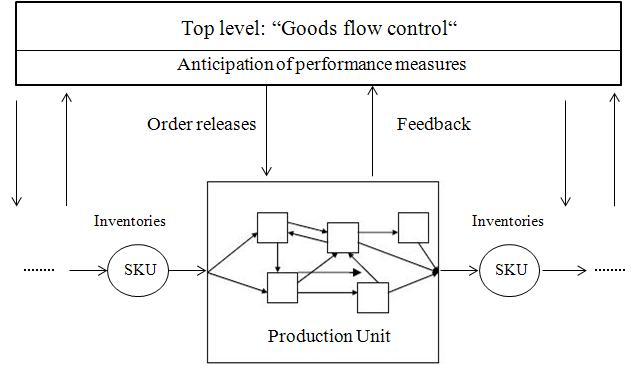
\includegraphics[width=0.65\textwidth]{figures/betrand.jpg}
%     %       \caption{ }
%     \end{figure}
%     \vspace{-1cm}

%     {\hfill \tiny Source:~\cite{Bertrand1990}.}
%   %   \end{minipage}

% \end{frame}

% \begin{frame}[t]
%   \frametitle{Average Reward}


% \end{frame}


% \begin{frame}[t]
%   \frametitle{Manufacturing Planning and Control Planning}

%   \begin{block}{Planning Parameters}
%     \begin{itemize}
%     \item Setting of planning parameters crucial
%     \item One key parameter is the lead time
%     \end{itemize}
%   \end{block}
%   \footnotetext{\cite{Bertrand1990}.}

%   \begin{definition}[Lead Time]
%     \alert{Lead time} (LT) is \alert{planned time} between release of an order and arrival in
%     finished goods inventory.
%   \end{definition}
%   \pause

%   \begin{definition}[Flow Time]
%     \alert{Flow time} is \alert{actual time} between release of an order and its completion. Consist of
%     processing, setup, control, transport, and waiting times.
%   \end{definition}
% \end{frame}

% % \begin{frame}[t]
% %   \frametitle{Waiting Times}

% %   \begin{block}{Waiting Times}
% %     \begin{itemize}
% %     \item Governing factor of flow time
% %     \item Result from queuing
% %     \item Depend heavily on amount of jobs in the system (WIP)
% %     \item Are subject to fluctuations due to variability in the system \MS[t]{soll ich das weg tun?}
% %     \item Difficult to estimate
% %     \end{itemize}
% %   \end{block}

% % \end{frame}

% \begin{frame}[t]
%   \frametitle{Order Release Decision}

%   \begin{block}{Order Release Decision}
%     \begin{itemize}
%     \item Determine nr. of orders to be released at beginning of period
%       \only<1-1>{\vspace{1.4325cm}}
%       \only<2->{\item Goal: Minimal costs
%       \begin{itemize}
%       \item Low Inventory $\rightarrow$ Short flow times $\rightarrow$ Timely completion
%       \item Nonlinear relationship between flow times and utilization
%       \end{itemize}
%     }
%     \end{itemize}

%     \vspace{-0.3cm}
%     \only<1-2>{
%     \begin{figure}[ht]
%       \centering
%       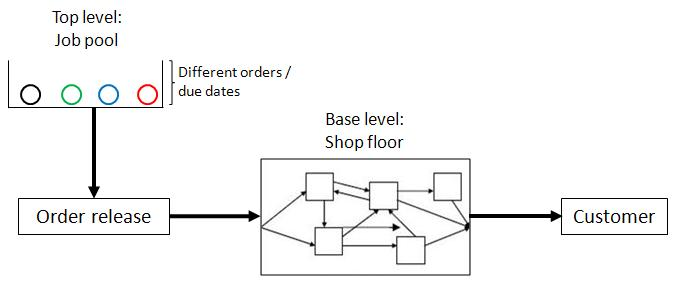
\includegraphics[width=0.91\textwidth]{figures/order_release.jpg}
%         %       \caption{Source: \MS[t]{TODO}}
%     \end{figure}
%   }
%     \only<3->{
%     \begin{figure}[ht]
%       \centering
%       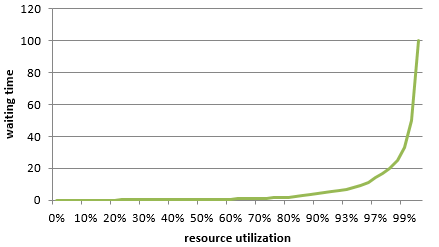
\includegraphics[width=0.70\textwidth]{figures/waiting_time_utilization.png}
%         %       \caption{Source: \MS[t]{TODO}}
%     \end{figure}

%   }

%   \end{block}


% \end{frame}


% \begin{frame}[t]
%   \frametitle{Lead Time Implications}

%   \begin{block}{Lead Time for Order Release Decision}
%     \begin{itemize}
%     \item Use lead time for order release decision. \pause
%     \item Common approach: Set static lead times. \pause
%     \item BUT: Should be set dynamically to react to dynamic operational characteristics of the
%       production process\footnotemark.
%       \pause
%     \item Solely reactive approach may lead to perpetually increasing flow times and poor
%       performance (Lead Time Syndrome) \pause
%       %       often generates an erratic release pattern (Lead Time Syndrome)
%     \item $\Rightarrow$ Predictive lead time management needed
%       %       Anticipation function for flow time is needed
%       \begin{enumerate}
%       \item Forecast the future performance as a function of the order release decision
%       \item Identify and avoid pathological behavior
%         %       \item Generate necessary corrective actions to prevent the LTS
%       \end{enumerate}
%     \end{itemize}
%     %   \end{block}
%   \footnotetext{\cite{hoyt1978dynamic,Selcuk2006}}

%     %   \begin{block}{}
%     \pause
%     \centering
%     \alert
%     {Adaptive order release mechanism based on RL}
%   \end{block}
% \end{frame}


% \begin{frame}[t]
%   \frametitle{Neural Network Setup}

%   \begin{block}{Neural Network Setup (Manually optimized)}
%     \begin{itemize}
%     \item Two three layer fully-connected networks
%     \item Both use 41-ReLU-89-ReLU-20-ReLU-9, with output activations being
%       \begin{itemize}
%       \item Softmax (normalized exponential) -- action probabilities
%       \item Tanh (hyperbolic tangent) -- expected discounted/avg reward
%       \end{itemize}
%     \end{itemize}
%   \end{block}

%   %   \begin{block}{External Benchmark}
%   %     Backward infinite loading (\BIL{})~\footnotemark:
%   %     \begin{align*}
%   %     %       \text{Release period}_{\text{Order}} = \text{Due Date}_{\text{Order}} - LT_{p}
%   %       \text{Release period} = \text{Due Date} - LT
%   %     \end{align*}
%   %     where $LT$ is static and predetermined.
%   %   \end{block}
%   %   \footnotetext{\cite{Ackerman1963}}


% \end{frame}


% \begin{frame}[t]
%   \frametitle{Workers}

%   \begin{block}{Workers}
%     \begin{itemize}
%     \item 20 workers
%     \item $w_{1}$ operates on learned policy
%     \item $w_{2},\ldots,w_{20}$:  random action with 20\% prob. or learned policy
%     \end{itemize}

%   \end{block}

% \end{frame}


% \begin{frame}[t]
%   \frametitle{Parameter Setup}

%   \begin{block}{Parameters}
%     \centering
%     \begin{tabular}{|l||c|c|c|c|c|c|c|}
%       \hline
%       Parameter & $p_{f}$ & $\gamma$ & $\alpha$ & $\tau$ & $N$ & $B$ \\
%       \hline
%       Value & 0.2 & 0.995\footnotemark & 0.95 & 0.001 & 30000 & 128 \\
%       \hline
%     \end{tabular}
%     \begin{tabular}{|l||c|c|c|}
%       \hline
%       Parameter & Train Iterations & Learn. Rate  & L2\\
%       \hline
%       Value & 4 & 0.01 & 0.0001\\
%       \hline
%     \end{tabular}
%   \end{block}

%   \begin{block}{Running Time}
%     The algorithm learned for 150k periods. The runtime for the evaluations was 1000 periods, with
%     750 periods startup phase and all evaluations were repeated 25 times.
%   \end{block}


% \end{frame}


% \begin{frame}
%   \begin{block}{Experimental Results II}
%     \centering
%     \begin{table}
%       \begin{tabular}{|l||c|c|c|c|c|c|c|c|c|}
%         %         BEGIN RECEIVE ORGTBL res2
%         \hline
%         Algorithm/KPI & SUM & % \%SL &
%         TARD & \(\sigma\)TARD & SFTT\\
%         \hline
%         %         Evaluation 1 & \multicolumn{11}{c|}{} \\
%         \ActShippedAvgRL    & \cellcolor{lightgray} 464.84 & 1.80 & 2.57 & 4.35 \\
%         \ActShippedAvg      & \cellcolor{lightgray} 473.46 & 1.87 & 2.79 & 3.13 \\
%         \ActOrdPool         & \cellcolor{lightgray} 497.83 & 1.92 & 2.84 & 4.23 \\
%         \BILThree       & 535.45 & 2.06 & 2.99 & 4.41 \\
%         \BILTwo         & \cellcolor{lightgray} 644.85 & 2.28 & 3.27 & 4.39 \\
%         \ActShipped     & \cellcolor{lightgray} 657.85 & 2.33 & 3.33 & 4.84 \\
%         \BILOne         & 803.74 & 2.49 & 3.65 & 4.39 \\
%         \ActRelOrds     & 896.51 & 2.46 & 3.64 & 4.21 \\
%         \hline
%         %         \multicolumn{8}{|l|}{\hspace{1.0cm}\new{\scriptsize{$^{\star}$The p-value of the comparison between
%         %         \ActShippedAvg{} and \ActOrdPool{} is $0.07364$}}}\\
%         %         \hline
%         %         RLN & 100 & 100 & 100 & 100 & 100 & 100 & 100 & 100 & 100 & 100 \\
%         %         \hline
%         %         Evaluation 2 & \multicolumn{11}{c|}{} \\
%         %         ImRe &  &  &  &  &  &  &  &  &  &  & \\
%         %         BILOne &  &  &  &  &  &  &  &  &  &  & \\
%         %         BILTwo &  &  &  &  &  &  &  &  &  &  & \\
%         %         BILThree &  &  &  &  &  &  &  &  &  &  & \\
%         %         BILTwo/4 &  &  &  &  &  &  &  &  &  &  & \\
%         %         RL & 100 & 100 & 100 & 100 & 100 & 100 & 100 & 100 & 100 & 100 & 100 \\
%         %         \hline
%         %         END RECEIVE ORGTBL res2
%       \end{tabular}
%     \end{table}
%     \begin{minipage}[t]{\textwidth}
%       \vspace{-0.5em} \centering {\footnotesize Evaluation results for sum of costs (SUM), tardiness
%       in \% and standard deviation (TARD, $\sigma$TARD) and shop floor throughput time (SFTT).}
%     \end{minipage}

%   \end{block}
% \end{frame}


% \begin{frame}[t]
%   \frametitle{Problems in OR}

%   \begin{block}{Problems in Operation Research Domain}
%     \begin{itemize}
%     \item Periodic and discrete decisions
%     \item Maximizing profits
%     \item High degree of complexity
%     \end{itemize}
%   \end{block}

% \end{frame}


\end{document}


%%% Local Variables:
%%% mode: latex
%%% TeX-master: t
%%% End:
